\documentclass[conference]{IEEEtran}
\IEEEoverridecommandlockouts
\usepackage{cite}
\usepackage{amsmath,amssymb,amsfonts}
\usepackage{algorithmic}
\usepackage{graphicx}
\usepackage{textcomp}
\usepackage{xcolor}
\usepackage{kotex}
\usepackage{tabularx}
\usepackage{supertabular,booktabs}
\usepackage{adjustbox}
\usepackage{enumitem}
\usepackage{romannum}
\usepackage{makecell}
\usepackage{multirow}
\usepackage{graphics}
\usepackage{subfigure}
\usepackage{float}
\usepackage{booktabs}
\usepackage{array}
\def\BibTeX{{\rm B\kern-.05em{\sc i\kern-.025em b}\kern-.08em
    T\kern-.1667em\lower.7ex\hbox{E}\kern-.125emX}}

\begin{document}
\pagestyle{plain}
\pagenumbering{arabic}

\title{COVER \\
- From Past to Present:\\
Harnessing Matter to Integrate Legacy Devices\\
into the Next-Gen Smart Home Ecosystem\\
}

\author{\IEEEauthorblockN{SONG WOOJUNG}
\IEEEauthorblockA{\textit{Dept. Information System} \\
\textit{Hanyang University}\\
Seoul, Republic of Korea \\
opusdeisong@gmail.com}
\and
\IEEEauthorblockN{KWON KITAE}
\IEEEauthorblockA{\textit{Dept. Information System } \\
\textit{Hanyang University}\\
Seoul, Republic of Korea \\
jrinonamu@gmail.com}
\and
\IEEEauthorblockN{KIM JINA}
\IEEEauthorblockA{\textit{Dept. Information System} \\
\textit{Hanyang University}\\
Seoul, Republic of Korea \\
drjina02@gmail.com}
\and
\IEEEauthorblockN{YEO DAKYUM}
\IEEEauthorblockA{\textit{Dept. Information System } \\
\textit{Hanyang University}\\
Seoul, Republic of Korea \\
yeodakyum@gmail.com}
}

\maketitle

\begin{abstract}
In recent times, the global smart home market has seen remarkable expansion, projected to cross \$164 billion by 2028. Driven by the desire for convenience, security, and energy savings, we're witnessing sophisticated device integrations in our homes. However, this growth isn't without its challenges. The array of smart home devices from different brands has fragmented the user experience, leading to a maze of applications for device control. Many third-party apps, despite their intentions, often don't mesh seamlessly with central control devices like smartphones, a challenge evident in platforms such as Apple Home and Google Home App . Additionally, a significant number of devices still lack IoT integration, which challenges expanding smart home market. [1]\\
Addressing these challenges, we introduce the LG Cover, an innovative solution designed to bridge gaps in the smart home ecosystem. We suggest specialized integration for all LG devices, resurrecting legacy devices through the Matter protocol, and ensuring consistent user experience across various brands. This system supports the integration of both Matter and ThinQ devices, and also supports older devices based on IR technology, revitalizing its utility within modern smart home setups.\\
To facilitate seamless integration, the LG Cover adopt a structured setup process involving the registration of the hub to the ThinQ app and the Matter API device. ThinQ supporting or IR supporting devices are connected to LG Cover with proprietary protocols, and LG Cover mediates the connected devices to Matter enabled controllers. Users are enabled to communicate with non-Matter-supporting devices through LG Cover using Matter API. With LG Cover's comprehensive approach, users can experience the convenience of a unified smart home ecosystem, irrespective of the device's age or brand.
\end{abstract}

\newpage

\large{Role Assignments}
\begin{table}[H]
\center
\begin{tabular}{m{1.7cm} m{1.4cm} m{4.0cm}}
\toprule
Roles & Name & Description\\
\midrule
User/Customer & SONG WOOJUNG &User/Customer plays the role of a various ages who needs support with an old LG devices that doesn’t support matter api. Despite the advancements in tech and the ubiquity of smart homes, not every device owned is compatible with the latest standards. This poses a challenge in achieving a cohesive experience, especially when most contemporary hubs primarily cater to the latest models and technologies. Therefore, the LG Cover plays an instrumental role in bridging this gap. While it is equipped to support the Matter API, its design philosophy is to be inclusive. The goal is to serve users like Alex, ensuring that their older, reliable LG devices don't become obsolete. This includes even those devices that don't support LG ThinQ.\\\\
Product Designer & KWON\ \ \ KITAE & A Product Designer is responsible for understanding user needs and business objectives to conceptualize and design products that provide effective solutions; they engage in user research to gather insights, sketch initial design ideas, create wireframes and interactive prototypes, collaborate with cross-functional teams like product managers, engineers, and marketers to refine designs, ensure consistency in brand aesthetics and user experience across products, gather and act on feedback from user testing sessions. Also works with documentation that helps other roles communicate with each other more effectively.\\\\
\bottomrule
\end{tabular}
\end{table}
\newpage

\begin{table}[H]
\center
\begin{tabular}{m{1.7cm} m{1.4cm} m{3.8cm}}
\midrule
Software developer & KIM JINA & A software developer is responsible for collaborating with development manager, product owners, and product designer to understand software requirements, converting these into functional specifications, designing the software architecture based on these requirements, writing clean and maintainable code, ensuring software is scalable and robust, testing the software for bugs and inconsistencies, deploying software to production environments, maintaining and updating software as necessary, and documenting development processes and software functionalities to ensure continuity and ease of future modifications. Also works with connection between the matter API and ThinQ devices to maintain connectivity.\\\\
Development manager & YEO DAKYUM & A Development Manager oversees the software development process, coordinating with cross-functional teams to ensure projects are completed on time and within budget, establishing and implementing development methodologies, setting objectives and deliverables for the development team, mentoring and providing guidance to developers, ensuring code quality and adherence to standards. Also works with the actual hardware chip that will be used in Cover.\\
\bottomrule
\end{tabular}
\end{table}

\section{\large{Introduction}}
\subsection{\large{Motivation}}
\begin{itemize}
\item Growth of Smart Home Systems\\
The smart home market has experienced remarkable growth over the last few years. According to Statista, the global smart home market is projected to surpass \$141 billion by 2023, up from \$76.6 billion in 2018. [2] This exponential growth is driven by consumers' increasing desire for convenience, security, and energy efficiency. As homes integrate more devices, the need for a cohesive control system becomes critical.\\
\item The Challenge of Diverse Devices from Different Companies \\
As smart home devices proliferate, a significant challenge arises due to the sheer variety of brands and products available. Different companies offer their distinct range of smart devices, each with its dedicated application for control. This leads to an overflow of applications on users' smartphones or tablets, complicating what should be a simplified process. [3][4] The fragmentation of control interfaces creates inefficiency and reduces the user-friendly nature of the smart home system. There's a clear need for a centralized platform, like Matter, that can consolidate control, ensuring that users can manage their entire smart home ecosystem without juggling multiple applications. \\
Additionally, there is a potential risk of user's personal information being exposed when remotely controlling products of diverse companies through IoT. Currently, when a user issues a command to turn on the lights from a mobile phone, it often goes through a cloud-based connection between the phone and the hub, and then the operation is executed via an API. [5] With Matter, all operations can be performed locally without passing through external servers, ensuring that personal information is not exposed.\\
\item Bridging the IoT Gap with LG Cover\\
While many modern devices are equipped with IoT capabilities, a substantial portion remains without this integration. The disparity between IoT-enabled devices and those lacking this feature can result in gaps within the smart home ecosystem. Matter, a unifying protocol for smart home devices, can introduce IoT capabilities to previously incompatible devices. LG Cover, supporting Matter, acts as a bridge, allowing even non-IoT devices to join the integrated smart home network. This inclusivity ensures that no device is left out, offering users a comprehensive smart home experience.\\
\end{itemize}

\subsection{\large{Problem Statement}}
\begin{itemize}
\item Gap in Dedicated Support for LG Devices\\
The landscape of smart home devices is increasingly complex and fragmented, with a myriad of brands and protocols available in the market. Within this expansive ecosystem, while there are many generic hubs available, there is a conspicuous absence of a dedicated hub designed specifically for LG's vast array of devices. Owners of LG products, both modern and legacy, find themselves in need of a hub that is acutely attuned to the nuances of LG's electronic architecture. Generic solutions often fall short in leveraging the full potential of LG devices, leaving users with a less-than-optimal experience.\\
\item Neglect of Legacy IR Devices and Old ThinQ Products\\
The tech industry's rapid advancement has led to a situation where many older, yet perfectly functional devices, especially those based on infrared (IR) technology and earlier versions of LG's ThinQ products, are left out of the modern smart home narrative. Most current hubs are squarely focused on the latest communication protocols, sidelining these older devices. This presents a challenge for many households that still rely heavily on these devices and are looking for ways to integrate them into a unified smart home ecosystem.\\
\item Diverse Brand Environment Leading to Fragmented User Experiences\\
The average household's smart device portfolio often comprises products from a variety of brands. Current IoT hubs, while claiming broad compatibility, tend to offer a disjointed user experience due to inconsistencies in how different brands' devices are integrated and managed. Users are thus left longing for a singular platform that can offer a seamless and harmonious experience across all their devices.\\
\end{itemize}

\subsection{\large{Solution}}
\begin{itemize}
\item Tailored Integration for LG's Spectrum of Devices\\
The LG Cover stands out with its commitment to providing a seamless experience specifically for LG device owners. Whether it's the latest smart TV or a legacy LG appliance, the LG Cover ensures perfect harmony and optimized performance, something that can only be achieved with a deep understanding of LG's technological DNA.\\
\item Inclusivity for Legacy Devices\\
One of LG Cover's hallmark features is its pioneering capability to revitalize older devices using the Matter protocol. Whether it's an IR-based remote-controlled device or an older iteration of the ThinQ product line, the LG Cover, through its integration with Matter, ensures that these devices are not only recognized but also seamlessly incorporated into the modern smart home ecosystem. By leveraging the universal nature of Matter, LG Cover effectively bridges the gap between past and present, preserving the utility and value of legacy devices in today's interconnected world.\\
\item Consistent Experience Across a Multitude of Brands\\
Beyond its specialization in integrating LG products, the LG Cover showcases its prowess in providing a consistent and intuitive interface, even when dealing with devices from multiple manufacturers. This focus on providing a unified user experience ensures that managing a diverse smart home setup is no longer a daunting task, but a delightful experience utilizing Matter, it would enable us to incorporate our device to many readily available, existing home management application, such as Apple HomeKit or Google Home App, which is much well suited for corresponding mobile OS.\\
\end{itemize}

\subsection{\large{Related Software}}
\begin{itemize}
\item Google Nest Hub 2 Gen.\\
Nest Hub is the device to use to manage your smart home since it is compatible with so many different things.\\
We can watch a range of movies, music, and TV shows using Nest Hub, and we can use voice commands or a single tap to operate connected smart devices. A sleep sensor function can also promote restful sleep.\\
Many Nest Hub functionalities are accessible through Quick Gestures. Quick Gestures uses Motion Sense instead of a camera to identify when our hand moves.\\
\item Samsung SmartThings Station\\
Samsung SmartThings Station combines a smart home hub and wireless phone charger while supporting up to three separate programmed automation routines.\\
It works with a broad selection of Matter and other Samsung smart home products, and its accompanying app makes it simple to set up routines you can activate from the Station with a tap.\\
It is incapable of playing music or supporting voice control because it lacks a speaker and microphone. Instead, this hub serves as a wireless charging station for devices that are Qi compliant.\\
Both the Android and iOS platforms currently support Samsung SmartThings Station.\\
\item SwitchBot Hub 2\\
SwitchBot Hub 2 supports old infrared appliances, we can link additional SwitchBot goods through Bluetooth and Wi-Fi to create a smart home environment.\\
We can integrate Hub 2 into our smart home ecosystem to deploy Matter over Wi-Fi in the future for current Bluetooth-only products like SwitchBot Curtain, SwitchBot Lock, and SwitchBot Blind Tilt, eliminating the need to purchase additional hardware to make them Matter compatible.\\
\item Ikea Dirigera Hub\\
DIRIGERA hub is the central control hub for a smart home in the IKEA Home smart app.\\
It enables us to connect and control a variety of smart gadgets, including speakers, blinds, and lighting. These devices allow for remote control, the creation of personalized settings for various situations and emotions, and the scheduling of automated chores.\\
We can operate your smart home using the app, remotes, voice commands, or motion thanks to the hub's flawless integration into our house's design. It is made to be user-friendly for everyone, including visitors, of all ages.\\
IKEA offers a growing selection of smart items to expand our setup over time and updates the app often to improve the smart home experience.\\
\item Bosch Smart Home Controller 2nd Gen.\\
Bosch Smart Home Controller II is a crucial part of the Bosch Smart Home ecosystem, serving as both hardware and software hub. It connects to various smart devices like thermostats and cameras and can integrate with third-party products. Users control it through a user-friendly app, web interface, or voice commands via popular voice assistants. It communicates using Wi-Fi, Zigbee, and Z-Wave.\\
Security and privacy are a priority with strong encryption. Regular updates enhance performance and security. It's energy-efficient and scales easily, making it the central unit for smart homes, providing control, security, and efficiency.\\
Smart Home Controller II ensures the security of our data, even when accessed remotely while we’re on the go. We have the flexibility to either control our system exclusively within our home network or remotely to monitor its status.\\
\item Homebridge\\
Homebridge is a lightweight NodeJS server that emulates the iOS HomeKit API. It allows users to integrate various smart home devices that do not natively support Apple’s HomeKit into the HomeKit ecosystem. Homebridge facilitates a broad array of plugins from various developers, which enables the connection and control of non-HomeKit devices via your iOS devices.\\
Being open-source software, Homebridge allows for transparency, community input, and modification. Users can delve into the code, understand how it works, and even contribute to its development. This openness fosters innovation and enables continuous improvement of the platform.\\
Its open-source nature, extensive plugin support, and active community make it a unique and invaluable tool for smart home enthusiasts, especially those invested in the Apple ecosystem.\\
\end{itemize}

\section{\large{Requirements}}
\subsection{\large{Installing Hub}}
\begin{enumerate}[label=\arabic*.]
\item {\large{Register LG Cover to ThinQ}}\\
To use non-Matter-supportive devices on home assistants as if they were Matter devices, LG Cover is to be registered to ThinQ app. The information regarding the device control function will be given to LG Cover to generate Matter-supportive QR code.\\
Registration procedure is as follows:\\
\begin{enumerate}[label=\alph*.]
\item In the ThinQ app, press ‘+’ to add new devices. A camera screen that reads QR codes appears.\\
\item Above the square frame for QR codes, click ‘matter’ button to add the LG Cover hub. \\
\item Read the QR code on LG Cover’s screen to register the hub to ThinQ app. \\
\item LG Cover is set to ThinQ app.\\
\end{enumerate}

\item {\large{Register LG Cover to Matter API device}}\\
LG Cover needs to be connected to user’s Matter API device to provide information from ThinQ app to home assistants such as Google Home, Apple Home, Alexa, and more. Matter API devices will recognize LG Cover as a Matter device and send or receive signals upon Matter protocols.\\
Registration procedure is as follows:\\
\begin{enumerate}[label=\alph*.]
\item In the home assistant application of the user’s device, execute menu for adding new devices.\\
\item Among the various ways and brands of devices, select ‘Matter’ or ‘Add Matter device’. A camera screen that reads QR codes appears. \\
\item Read the QR code on LG Cover’s screen and click “Add to Home Assistant”. \\
\item LG Cover is set to the user’s Matter API devices.\\
\end{enumerate}
\end{enumerate}

\subsection{\large{Register device to LG Cover}}
Devices registered to ThinQ app can be operated from user’s home assistant just like Matter devices via LG Cover. ThinQ and LG Cover is connected, and LG Cover, the bridge hub, mediates ThinQ and Matter API home assistants. Therefore, as users register their devices to Register devices to LG Cover using one of the following three methods according to the supported module for the device.\\
\begin{enumerate}[label=\arabic*.]
\item {\large{Matter device}}\\
All matter devices use setup code, which is provided on the device, in the packaging, or in an app. Register the Matter device to ThinQ to control device though LG Cover. Matter devices can be registered to the Matter API device through ThinQ or directly to home assistants.\\
Registration procedure is as follows:\\
\begin{enumerate}[label=\alph*.]
\item In the ThinQ app, press ‘+’ to add new devices. A camera screen that reads QR codes appears.\\
\item Above the square frame for QR codes, click ‘matter’ button to add device.\\
\item Read the QR code on the device to register the device to ThinQ app. \\
\item Click “Connect through NFC” or “Connect through Pin” to connect the device by tapping on the NFC tag or manually entering the setup digits.\\
\item Device is registered to ThinQ.\\
\end{enumerate}
Registration procedure to home assistant is as follows:\\
\begin{enumerate}[label=\alph*.]
\item Read the QR code on the device.\\
\item Page will be redirected to registration page for home assistant app.\\
\item Click “Add to Home Assistant”. \\
\item Device is registered to Matter API home assistant.\\
\end{enumerate}

\item {\large{ThinQ device}}\\
LG appliances that support ThinQ can be registered easily on the app.  Devices connected to ThinQ are automatically added to Matter devices via LG Cover acting as a bridge. Register the device to ThinQ to manage the device from home assistants through LG Cover.\\
Registration procedure is as follows:\\
\begin{enumerate}[label=\alph*.]
\item In the ThinQ app, press ‘+’ to add new devices. A camera screen that reads QR codes appears.\\
\item Read the QR code of the device or find the device from the list of products provided.\\
\item Device is registered to ThinQ app.\\
\end{enumerate}

\item {\large{Legacy Infrared(IR) device}}\\
Infrared supporting devices could or could not be LG’s products. If the device is not in LG’s database, IR signals should be recorded with IR receiver. If the device is LG’s product, IR signals would be listed in LG’s database. In this context, LG Cover must possess the capability to access the database of infrared signals associated with a particular device.\\
Devices that supports only infrared remote control can be registered to ThinQ and be managed by LG Cover.\\
Registration procedure is as follows:\\
\begin{enumerate}[label=\alph*.]
\item In the ThinQ app, click "Add device by IR". \\
\item ThinQ requests for IR signals.\\
\item User sends signals to LG Cover through remote controllers or any kind of IR controllers.\\
\item The name of the device will be set by smart matching or manually by user.\\
\item The device is registered to ThinQ.\\
\end{enumerate}
\end{enumerate}

\subsection{\large{Integration}}
LG cover is able to access ThinQ API via RESTful API. As new devices that do not support Matter protocol are registered to ThinQ app, LG Cover pulls users’s devices from ThinQ. The information can hold the name of the device and list of signals for device operation to be managed in Cover.\\
LG Cover receives information about the newly registered device. LG Cover is already linked to Matter API devices, or home assistants. Therefore, LG Cover mediates the newly registered device to home assistants and lets Matter API devices to recognize the device as a Matter-supporting device and communicate with the device using matter signals.\\
The user's actions to trigger these operations and the corresponding signal flow are as follows:\\
\begin{enumerate}[label=\arabic*.]
\item {\large{Matter device}}\\
Devices that support Matter can be controlled directly from home assistants using Matter API.\\

\item {\large{ThinQ device}}\\
Communication from user to device can be processed as following:\\
\begin{enumerate}[label=\alph*.]
\item User sends a Matter signal through home assistant.\\
\item LG Cover receives the Matter signal.\\
\item LG Cover delivers the command to ThinQ API by network.\\
\item ThinQ app receives the command from LG Cover and executes the command.\\
\end{enumerate}
Communication from device to user can be processed as following:\\
\begin{enumerate}[label=\alph*.]
\item Device sends a signal to ThinQ through network.\\
\item ThinQ receives the signal from device and LG Cover acquires the data from ThinQ API.\\
\item LG Cover translates the signal and delivers the data to home assistant by Matter signal.\\
\item Matter API device, home assistant, receives the data and conveys information.\\
\end{enumerate}

\item {\large{IR device}}\\
Communication from user to device can be processed as following:\\
\begin{enumerate}[label=\alph*.]
\item User sends a Matter signal through home assistant.\\
\item LG Cover receives signal via Matter.\\
\item LG Cover indicates the Matter signal and transmits the corresponding IR signal for IR device to receive.\\
\end{enumerate}
\end{enumerate}

\subsection{\large{Control device using LG Cover}}
\begin{enumerate}[label=\arabic*.]

\item {\large{Matter device}}\\
Matter devices provide simple and complicated control options available by Cover and home assistants.\\
Cluster is a group of functions, such as On/Off Cluster or Level Control Cluster. In general, user should be able to use a variety of clusters supported by home assistant, along with manufacturer-specified functions. Among the clusters supported by home assistant, some of the most common ones include On/Off, Open/Close, Color Control, Level Control, Temperature Measurement, and more.\\
Node encapsulates the full product and controls all endpoints of the particular device. Each endpoint includes clusters, and each cluster holds attributes and events.\\
Consider a device that belongs to On/Off Light Switch Device Type, and holds two endpoints. Endpoint 1 includes the Server On/Off Cluster, and Endpoint 2 includes the Client On/Off Cluster.\\
The flow of an On/Off control is as follows:\\
\begin{enumerate}[label=\alph*.]
\item User clicks the On/Off button from home assistant.\\
\item The Client Cluster controls the Server Cluster.\\
\item Server Cluster triggers the command to turn on or turn off the switch.\\
\begin{enumerate}[label=\roman*.]
\item If the OnOff attribute of the Node is “On”, the switch would be turned off.\\
\item If the OnOff attribute of the Node is “Off”, the switch would be turned on.\\
\end{enumerate}
\end{enumerate}

\item {\large{ThinQ device}}\\
Complicated control functions of appliances can also be added to Matter API device in forms of shortcuts. Cover enables user selected commands be registered as shortcuts in the device, and user is able to execute the command by just one click.\\
Simple Control:\\
\begin{enumerate}[label=\alph*.]
\item Turn On / Turn Off\\
User can turn on and turn off the matter device from home assistants by clicking “On/Off” button from the home assistant app or from user defined shortcuts.\\
\end{enumerate}
Complicated Control:\\
\begin{enumerate}[label=\alph*.]
\item Refrigerator Temperature\\
User can check the temperature of each section through home assistants.\\
User can set the temperature to personal preference through home assistants.\\
\item Washing Machine\\
Washing mode, water temperature, number of rinse, and other control functions can be set with home assistants.\\
\end{enumerate}

\item {\large{IR device}}\\
\begin{enumerate}[label=\alph*.]

\item LG product\\
LG holds information of all LG products. Therefore, all commands of IR devices are available even if the device does not support ThinQ. When LG IR device is registered to ThinQ through LG Cover, ThinQ can manage several commands of the device with LG Cover for Matter controls.\\
Simple Control:\\
\begin{enumerate}[label=\roman*.]
\item Turn On / Turn Off\\
User can turn on and turn off the matter device from home assistants by clicking “On/Off” button from the home assistant app or from user defined shortcuts.\\
\end{enumerate}
Complicated Control:\\
\begin{enumerate}[label=\roman*.]
\item Air conditioner
\begin{enumerate}
\item Wind direction\\
Direction of the be wind, from top to bottom, left to right, can set through home assistants.\\
\item Wind temperature\\
Increase and decrease in wind temperature can be set through home assistants.\\
\item Operation Mode\\
Operation mode such as Air-conditioning, dehumidification, and heating can be set through home assistants.\\
\end{enumerate}
\item TV
\begin{enumerate}
\item Remote Controller\\
Sound, channels, and other control functions can be set with home assistants.\\
\end{enumerate}
\end{enumerate}

\item Non-LG product\\
Information of IR devices of other manufacturers is not available by LG. Therefore, when the device is registered to ThinQ through LG Cover, information to be sent is very limited. Only simple control functions can be registered to Cover.\\
\begin{enumerate}[label=\roman*.]
\item Turn On / Turn Off\\
User can turn on and turn off the matter device from home assistants by clicking “On/Off” button from the home assistant app or from user defined shortcuts.\\
\end{enumerate}

\end{enumerate}

\end{enumerate}


\section{\large{Development Environment}}

\subsection{\large{Choice of hardware development environment}}
\begin{itemize}
\item Consideratoins for Matter\\
\begin{figure}[H]\centering 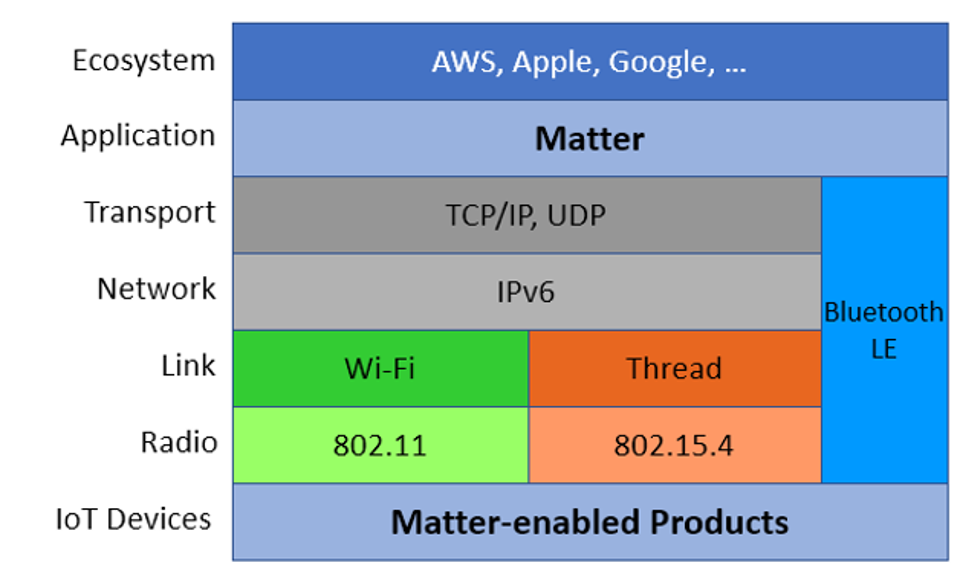
\includegraphics[scale=0.25]{images/consideratoins-matter.png}\end{figure}
\item Requirements for Matter\\
As you can see from Matter’s formal name CHIP (Connected home IP) it runs on existing IP. However, there is bit of difference in PHY layer that it could use Thread running on IEEE 802.15.4 radio instead of WiFi on IEEE 802.11 radio.\\
For Matter enabled devices and especially a Matter hub that connects with various devices, most likely it would require 802.11, 802.15.4 and BLE connectivity.  It would be very cost prohibitive and detrimental to implement various radios one by one with generic off the shelf 8 bit microcontroller such as AVR or PIC, and workload required for matter is questionable for it to run on old, almost deprecated 8bit MCUs of past. While we could use 32 bit microcontroller such as ARM cortex lineup to solve the processor performance issue, it would still leave the issue of having to implement such radios.\\
It would be much better off with dedicated SoC with everything needed implemented, ready to go. While designing customized chip is completely outside of this scope, thankfully there already exists a MCU supporting Wifi, Thread, and BLE in one single convenient package; ESP32 series.\\
\item ESP32\\
ESP32 is a series of low-cost, low-power system on a chip microcontrollers with integrated Wi-Fi and dual-mode Bluetooth. The ESP32 series employs either a Tensilica Xtensa LX6 microprocessor in both dual-core and single-core variations, Xtensa LX7 dual-core microprocessor or a single-core RISC-V microprocessor and includes built-in antenna switches, RF balun, power amplifier, low-noise receive amplifier, filters, and power-management modules. ESP32 is created and developed by Espressif Systems, a Chinese company based in Shanghai, and is manufactured by TSMC using their 40 nm process. It is a successor to the ESP8266 microcontroller.\\
Since the release of the original ESP32, a number of variants have been introduced and announced. They form the ESP32 family of microcontrollers. These chips have different CPUs and capabilities, but all share the same SDK and are largely code-compatible.\\
A minimal table to compare the Espressif's MCU families.\\
\\\\\\\\\\\\
\item Comparison of ESP32, ESP32-S3, and ESP32-C6
\setlength{\extrarowheight}{2.5pt}
\begin{table}[H]
\centering
\begin{tabular}{|m{1.8cm}|m{1.8cm}|m{1.8cm}|m{1.8cm}|}
\hline
\textbf{Model} & \textbf{ESP32} & \textbf{ESP32-S3} & \textbf{ESP32-C6} \\
\hline
\textbf{Announcement Date} & 2016, September & 2020, December & 2021, April \\
\textbf{Main processor} & Tensilica Xtensa 32-bit LX6 (up to 240MHz) (optionally dual core) & Tensilica Xtensa 32-bit LX7 dual core (up to 240MHz) & RISC-V 32-bit (up to 160MHz) \\
\textbf{SRAM} & 520KB & 512KB & 400KB \\
\textbf{ROM} & 448KB & 384KB & 384KB \\
\textbf{JTAG} & O & ? & O \\
\textbf{Cache} & 64KB & ? & ? \\
\textbf{WiFi} & Wi-Fi 4 & Wi-Fi 4 & Wi-Fi 6 \\
\textbf{Bluetooth} & BLE 4.2 (upgrade to 5.0, with limitations) & BLE 5.0 & BLE 5.0 \\
\textbf{Ethernet} & O & ? & ? \\
\textbf{RTC memory} & 16KB & 16KB & ? \\
\textbf{PMU} & O & ? & ? \\
\textbf{ULP coprocessor} & O & ? & ? \\
\textbf{Cryptographic Accelerator} & SHA, RSA, AES, RNG & SHA, RSA, AES, RNG, HMAC, Digital Signature & SHA, RSA, AES, RNG, HMAC, Digital Signature \\
\textbf{Secure boot} & O & O & O \\
\textbf{Flash encryption} & O & O & XTS-AES-128 \\
\textbf{SPI} & 4 & ? & ? \\
\textbf{I2C} & 2 & ? & ? \\
\textbf{I2S} & 2 & ? & ? \\
\textbf{UART} & 3 & ? & ? \\
\textbf{SDIO Host} & 1 & 2 & 0 \\
\textbf{SDIO Slave} & 1 & 0 & 0 \\
\textbf{GPIO} & 34 & 44 & 22 \\
\textbf{LED PWM} & 16 & ? & ? \\
\textbf{MCPWM} & 6 & 2 & 0 \\
\textbf{Pulse counter} & 8 & ? & X \\
\textbf{GDMA*} & 0 & ? & ? \\
\textbf{USB} & X & ? & ? \\
\textbf{TWAI**} & 1 & ? & ? \\
\textbf{ADC} & 2x 12-bit SAR, up to 18 channels & ? & ? \\
\textbf{DAC} & 2x 8-bit & ? & X \\
\textbf{RMT} & 8x transmission/reception & ? & ? \\
\textbf{Timer} & 4x 64-bit & ? & ? \\
\textbf{Temperature Sensor} & O & ? & ? \\
\textbf{Hall Sensor} & O & ? & ? \\
\textbf{Touch Sensor} & 10 & ? & ? \\
\hline
\end{tabular}
\end{table}


While ESP32-C6 seems like a best choice since it has 802.15.4 capability, It is currently logistically difficult to get a development board. So we had to opt for ESP32-S3, while lacking 802.15.4 support, as current state of 802.15.4 Thread have long way to go before going mainstream we concluded it was not vital.\\
\end{itemize}

\textbf{ESP32-S3} is a dual-core XTensa LX7 MCU, capable of running at 240 MHz. Apart from its 512 KB of internal SRAM, it also comes with integrated 2.4 GHz, 802.11 b/g/n Wi-Fi and Bluetooth 5 (LE) connectivity that provides long-range support. It has 45 programmable GPIOs and supports a rich set of peripherals. ESP32-S3 supports larger, high-speed octal SPI flash, and PSRAM with configurable data and instruction cache.\\
As we are not just building a virtual docker image, there is some considerations that have to be made.\\

\begin{itemize}
\item ESP32-S3 module\\
ESP32-S3 comes in different form factors, but there is mainly two. One being just a bare chip in QFN56 package, and another being with basic components laid out in PCB with antenna and RF shield. \\
\begin{enumerate}[label=\arabic*.]
\item ESP32-S3
\begin{figure}[H]\centering 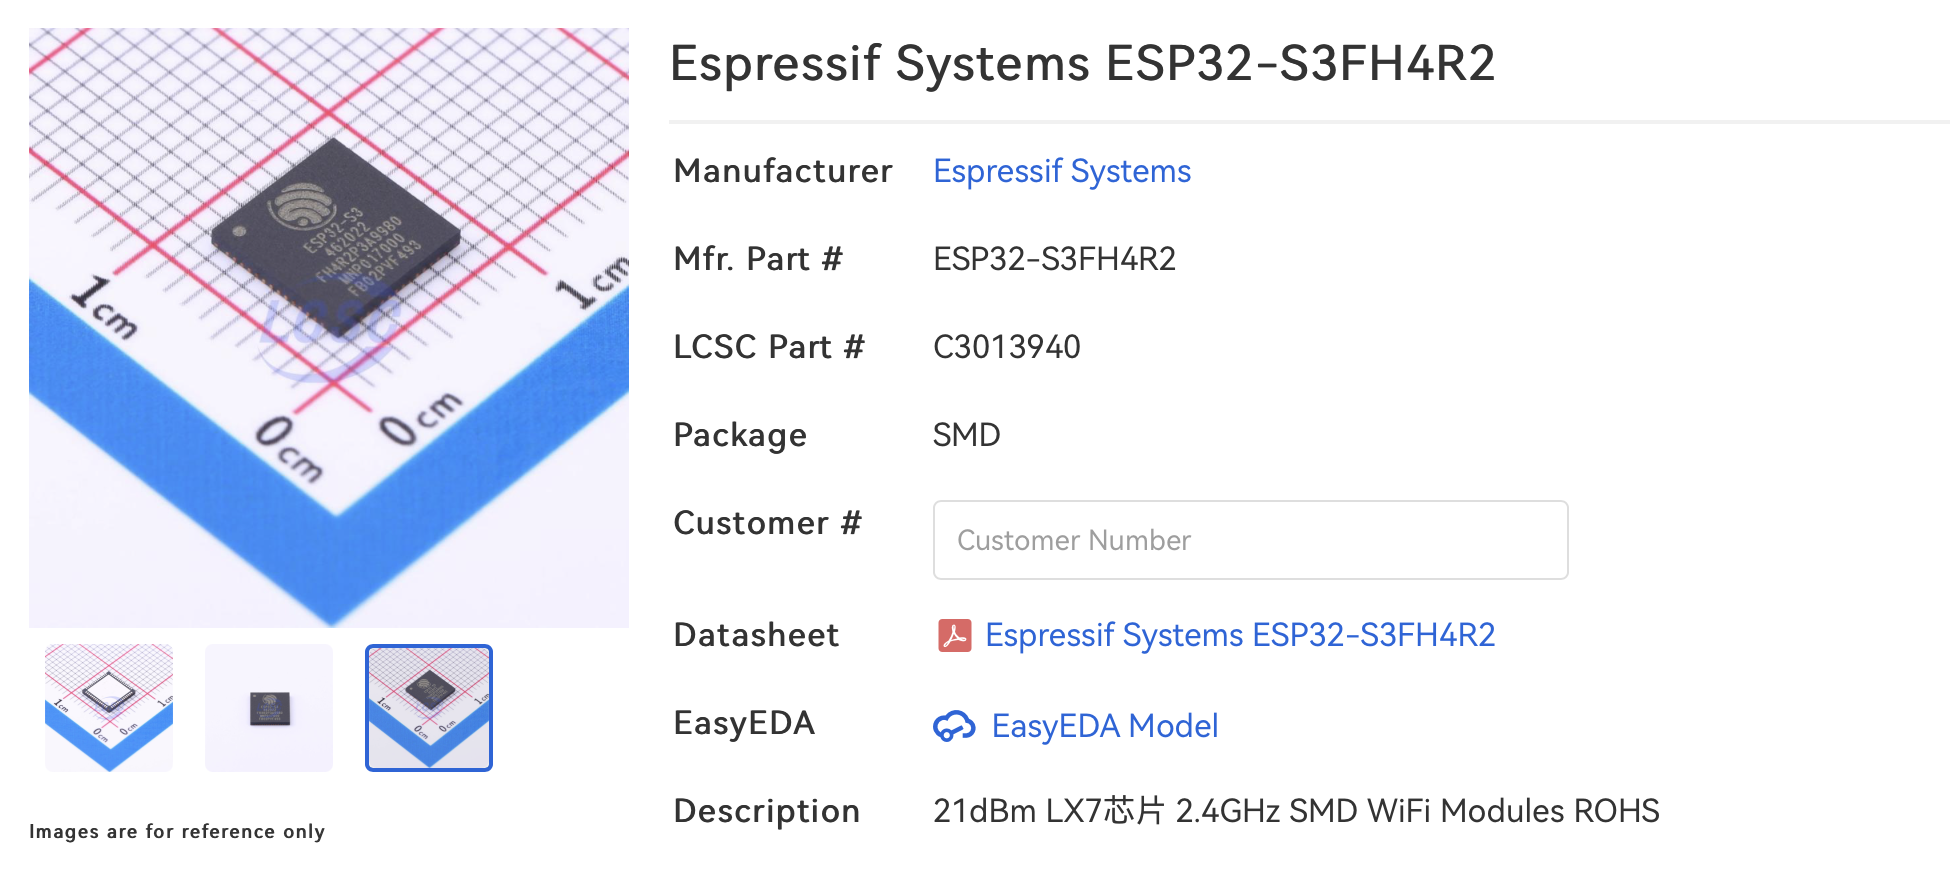
\includegraphics[scale=0.25]{images/esp32-s3.png}\end{figure}
\begin{itemize}
\item very difficult to design RF PCB\\
\item could lead to sub-optimal design\\
\item not FCC certified\\
\end{itemize}
\item ESP32-S3-WROOM-1
\begin{figure}[H]\centering 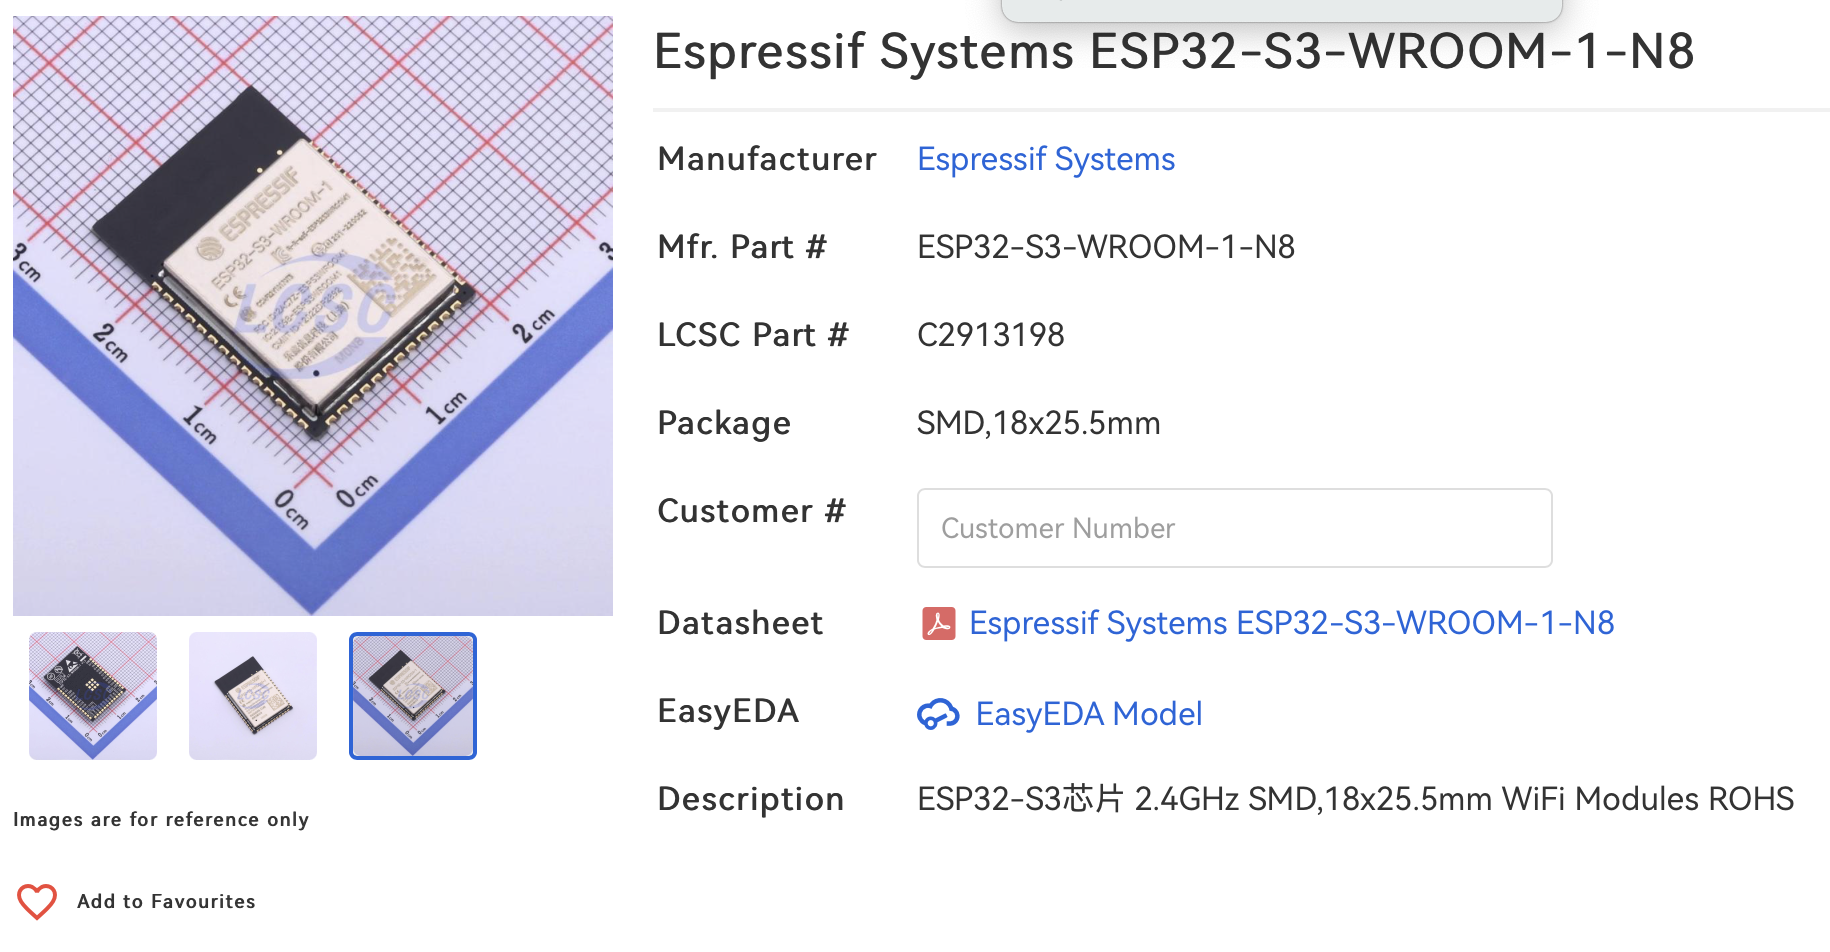
\includegraphics[scale=0.25]{images/esp32-s3-wroom-1.png}\end{figure}
\begin{itemize}
\item Easier to implement\\
\item have ready made pcb / rf shield\\
\item FCC certified\\
\item easier to meet local RF regulation laws\\
\end{itemize}
\end{enumerate}

\begin{table}[H]
\centering
\begin{tabular}{lcccr}
\toprule
Ordering Code          & Flash            & PSRAM          \\
\midrule
ESP32-S3-WROOM-1-N4    & 4 MB (Quad SPI)  & -              \\
ESP32-S3-WROOM-1-N8    & 8 MB (Quad SPI)  & -              \\
ESP32-S3-WROOM-1-N16   & 16 MB (Quad SPI) & -              \\
ESP32-S3-WROOM-1-H4    & 4 MB (Quad SPI)  & -              \\
ESP32-S3-WROOM-1-N4R2  & 4 MB (Quad SPI)  & 2 MB (Quad SPI)\\
ESP32-S3-WROOM-1-N8R2  & 8 MB (Quad SPI)  & 2 MB (Quad SPI)\\
ESP32-S3-WROOM-1-N16R2 & 16 MB (Quad SPI) & 2 MB (Quad SPI)\\
ESP32-S3-WROOM-1-N4R8  & 4 MB (Quad SPI)  & 8 MB (Octal SPI)\\
ESP32-S3-WROOM-1-N8R8  & 8 MB (Quad SPI)  & 8 MB (Octal SPI)\\
ESP32-S3-WROOM-1-N16R8 & 16 MB (Quad SPI) & 8 MB (Octal SPI)\\
\bottomrule
\end{tabular}
\end{table}

\end{itemize}

\begin{itemize}
\item Wi-Fi + Bluetooth 5 (LE)\\
ESP32-S3 supports a 2.4 GHz Wi-Fi (802.11 b/g/n) with 40 MHz of bandwidth support. The Bluetooth Low Energy subsystem supports long range through Coded PHY and advertisement extension. It also supports higher transmission speed and data throughput, with 2 Mbps PHY. Both Wi-Fi and Bluetooth LE have superior RF performance that is maintained even at high temperatures.\\
\item Mature Software Support\\
ESP32-S3 is supported through Espressif’s popular ESP-IDF platform that already powers millions of devices on the market. ESP-IDF comes with rigorous testing, regular updates and an unparalleled support policy. Based on ESP-IDF’s mature software architecture, developers can easily build applications anew or migrate their own applications to the ESP32-S3 platform, and continue working with the trusted ESP-IDF tools and APIs.\\
\item Security\\
ESP32-S3 provides all the necessary security requirements for building securely connected devices, without requiring any external components. It supports AES-XTS-based flash encryption, RSA-based secure boot, digital signature and HMAC. ESP32-S3 also has a “World Controller” peripheral that provides two fully-isolated execution environments, which enables the implementation of a trusted-execution environment or a privilege-separation scheme.\\
\end{itemize}

\subsection{\large{Choice of software development platform}}
\begin{enumerate}[label=\arabic*.]
\item Development Platform\\
\begin{enumerate}[label=\alph*.]
\item Linux\\
Linux is based on the Unix operating system which supports a wide range of programming languages, tools, and frameworks. The operating system is used for server environments, desktop applications, and embedded systems development, among others. Linux's command-line utilities are particularly well-suited for working with development boards and IoT devices. Linux is apt for IoT development due to its performance and the extensive community support available for troubleshooting and enhancements.\\
\item macOS Monterey\\
macOS Monterey is Apple Inc.'s desktop operating system for Macintosh computers. It is compatible with many development tools, languages, and frameworks essential for different kinds of software development, including web development, mobile app development, and hardware programming.\\
\end{enumerate}

\item Language and Framework\\
\begin{enumerate}[label=\alph*.]
\item Espressif ESP-IDF\\
ESP-IDF is Espressif’s official IoT Development Framework for the ESP32, ESP32-S, ESP32-C and ESP32-H series of SoCs. It provides a self-sufficient SDK for any generic application development on these platforms. ESP-IDF currently powers millions of devices in the field, and empowers building a variety of network-connected products, ranging from simple light bulbs to big appliances and industrial devices. ESP-IDF runs on the FreeRTOS operating system, with modifications to better support the SoC's features and capabilities. It uses C as the programming language and provides a suite of development tools for flashing the SoC, monitoring output, and debugging. Various components, component level configuration, and command line support of ESP-IDF enables developers to build their projects at ease. [6]\\
\begin{figure}[H]\centering 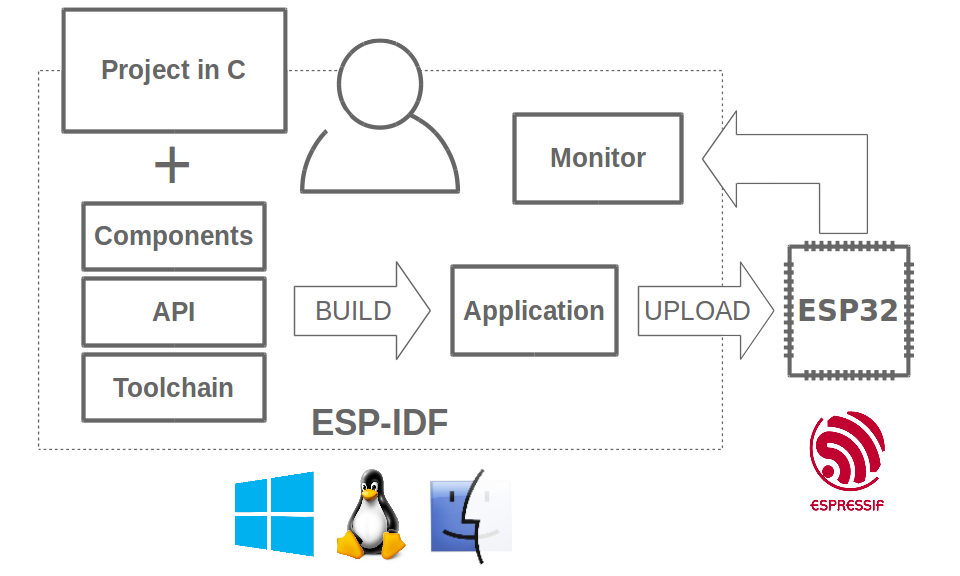
\includegraphics[scale=0.33]{images/esp-idf.png}\end{figure}
\item C/C++\\
C is a procedural high-level programming language that is designed to provide efficient access to memory and language constructs that map efficiently to machine instructions. C++ supports both procedural and object-oriented programming paradigms, and provides features such as overloading, templates, and exceptions, which are not available in C. The core components of ESP-IDF and the APIs provided for interacting with the ESP32 hardware are written in C. This allows for efficient interaction with the hardware and is suitable for the resource-constrained environments typically associated with embedded systems. The framework provides support for C++ exceptions and other features, allowing developers to leverage the object-oriented aspects of C++ in their ESP32 projects.\\
\item xtensa-esp-elf\\
xtensa-esp-elf is a toolchain for 32-bit Xtensa microcontrollers, based on GCC. It provides all the necessary tools to transform high-level code into a binary form that the microcontroller can execute, handling the specifics of the Xtensa architecture, including its custom instructions and configurations. xtensa-esp-elf includes a collection of binaries such as an assembler, linker, and archiver that prepare the code for execution on the microcontroller. The compiler, extensa-esp-elf-gcc, is the customized version of GCC provided by Espressif, tailored specifically for the Xtensa architecture of ESP32 and ESP32-S series. It allows developers to compile C and C++ code into efficient machine language that can run directly on the low-level hardware. This version of GCC has been optimized to harness the unique features and capabilities of the ESP32's processor, ensuring that developers can maximize performance for a variety of applications, from simple IoT devices to complex networking systems, while leveraging the rich set of features and the robust development framework provided by ESP-IDF. Since the Xtensa cores are different from the architecture of a typical development computer (x86\_64 or arm), the xtensa-esp-elf-gcc performs cross-compilation, generating executable code for a different architecture than that of the build host. The xtensa-esp-elf toolchain is versatile and supports development across multiple operating systems, including Linux, macOS, and Windows, thus enabling a wide range of developers to create applications for Espressif's hardware platforms regardless of their preferred development OS. [7]\\
\item CMake\\
CMake is a cross-platform, open-source build system generator widely used for managing the build processes of software in a compiler-independent manner. It enables developers to define build configurations using simple, platform- and compiler-agnostic configuration files, known as makefile. The primary function of CMake is to control the software compilation process using simple platform and compiler-independent configuration files to generate native makefiles or project files that can be used in the compiler environment of your choice. CMake supports out-of-source builds, allowing for multiple build types to be generated from a single source tree and facilitating cleaner build directories and easier maintenance. It is equipped to handle large projects spanning multiple directories and can also manage complex dependency chains between components. With its ability to target various platforms and its extensive scripting capabilities, CMake has become a go-to tool for developers looking to streamline their build processes and improve portability and scalability of their software projects. [8]\\
\item Ninja\\
Ninja is a small build system with a focus on speed. It takes as input the build files generated by tools like CMake and executes the build as efficiently as possible. Unlike CMake, which is a build system generator, Ninja is the actual build system that does the compiling, linking, and other build steps. Ninja aims to outperform other build systems by using simple build files and aggressively caching intermediate build results to minimize redundant work. This design philosophy makes Ninja particularly well-suited for large codebases and for continuous integration systems where build times can significantly affect the development workflow. Although Ninja is not designed to be written by humans directly, its simplicity and high performance have made it an attractive backend for build system generators that prioritize speed and efficiency. [9]\\
\item React Native\\
React Native is an open-source framework developed by Facebook for creating native-style mobile apps using React and JavaScript. It enables developers to build applications for multiple platforms, including iOS and Android, with a single codebase, leveraging a rich ecosystem of libraries and tools. Its component-based structure allows for the reuse of code across different platforms, while maintaining the ability to integrate with native functionality and third-party libraries. The framework's live and hot reloading capabilities significantly enhance developer productivity, and its large community provides strong support, with contributions extending its reach to platforms like Windows and macOS. Given these benefits, a significant number of developers opt for React Native to create mobile applications that deliver a native user experience with the agility of web app development. [10]\\
\item Go\\
Go, often referred to as Golang, is a programming language created at Google and derived from the syntax of the C language, aiming to make development simple, efficient, and readable. The language supports a wide array of programming paradigms, including concurrent, functional, and object-oriented styles. Go is used for backend systems, cloud computing, and DevOps tools, and others. Go's built-in concurrency support, along with its powerful standard library and garbage collection, makes it particularly well-suited for building fast, scalable network servers and distributed systems. Owing to Go’s supporting features, Go has become a preferred choice among developers for managing backend systems. [11]\\
\end{enumerate}
\end{enumerate}

\subsection{\large{Software in use}}
\begin{enumerate}[label=\arabic*.]
\item LG ThinQ, LG SmartHome Application\\
The LG ThinQ app is a smart application designed to connect, manage, and communicate with LG smart appliances, providing users with a seamless and intuitive way to ensure their devices operate smoothly. It allows for remote monitoring and control of LG appliances, offering features such as laundry cycle tracking, refrigerator management, and the ability to send cooking instructions to ovens. Integration with voice assistants like Google Assistant and Alexa further enhances the user experience, enabling voice commands for convenience. The app's Smart Diagnosis and proactive alerts system aid in maintaining appliance health, alerting users to potential issues and facilitating troubleshooting. Additionally, ThinQ UP feature keeps appliances up-to-date with the latest software, allowing for personalization and enhanced functionality tailored to users' lifestyles and preferences, underscoring LG's commitment to smart home innovation and user-centric design. [12]\\
\item VSCode (Visual Studio Code)\\
Visual Studio Code (VSCode) is a free, open-source code editor developed by Microsoft, renowned for its performance, extensibility, and support for a wide range of programming languages and tools. It combines simplicity with powerful developer tooling, like built-in Git commands, a robust debugging suite, and IntelliSense for smart code completion. Its lightweight design ensures smooth operation, while extensions available through its marketplace allow developers to customize and enhance their coding environment to suit a multitude of workflows. This flexibility, coupled with features like live share for collaborative coding and a built-in terminal, has made VSCode a popular choice among developers across disciplines, from web development to data science and beyond. [13]\\
\item GitHub\\
GitHub is a web-based platform that provides hosting for software development version control using Git, facilitating collaborative coding from contributors worldwide. It acts as a repository hosting service, allowing developers to share their code, track changes, and manage versions with robust version control and collaboration features. GitHub extends Git's functionality with its own features, such as issue tracking, feature requests, task management, continuous integration, and wikis for project documentation. It has become an essential tool for both open-source and private software projects, creating a community that fosters learning, sharing, and collaboration on a global scale. GitHub's impact is substantial, providing a nexus for software development and a repository for a vast array of projects across different fields and technologies.\\
\item Figma\\
Figma is a cloud-based design tool that specializes in user interface and user experience design with real-time collaboration. It stands out for its intuitive interface and vector-based graphics, which are pivotal in modern web and mobile application design. As a browser-based tool, it allows designers to work on projects from anywhere, share their work instantly, and receive feedback dynamically. Teams can simultaneously edit projects, significantly streamlining the design process. Figma supports the entire design journey—from wireframing to prototyping to delivering final assets—all within the same environment. Its component system and design libraries enable consistency across designs, while plugins and integrations enhance its functionality. This all-encompassing solution has made Figma a go-to tool for designers, product teams, and organizations looking to create and iterate on designs efficiently.\\
\item LaTeX\\
LaTeX is a high-quality typesetting system; it includes features designed for the production of technical and scientific documentation. It is the de facto standard for the communication and publication of scientific documents in many fields, including mathematics, computer science, engineering, physics, chemistry, and economics. LaTeX is based on the TeX typesetting system, and it excels at complex documents that contain a lot of mathematics, references, citations, and cross-referencing. Rather than focusing on the appearance of the document directly, it encourages authors to concentrate on its structure by defining commands that describe the logical structure of a document. These commands are compiled to produce a beautifully formatted document in PDF or other formats, with high typographical quality, suitable for academic and professional publication. LaTeX is widely used in academia for the submission of scientific papers and is available as free software.\\
\item Notion\\
Notion is an all-in-one workspace application designed to integrate notes, tasks, wikis, and databases into a single, user-friendly interface, promoting productivity and organization for both personal and professional use. It offers a highly flexible environment where users can create custom pages and databases with rich content types, such as text, images, checklists, and links, and connect these elements in a modular way. Notion's powerful organizational tools, including nested pages, tagging, and sorting, allow for detailed knowledge management and project tracking. Its collaborative features enable real-time teamwork and sharing, making it popular among remote teams, students, and individuals seeking a centralized platform to manage their work and studies. With its sleek design and versatile functionality, Notion stands out as a multifaceted tool that adapts to various workflows and simplifies the integration of diverse information and task management.\\
\end{enumerate}

\subsection{\large{Specification}}

\subsection{\large{Cost}}
\begin{table}[H]
\center
\begin{tabular}{m{1.7cm} m{1.4cm} m{1.4cm}}
\toprule
Name & Price & Quantity\\
\midrule
ESP32-S3 & 3 dollars &1\\\\
Laptop & 1000 dollars & 1\\\\
Apple TV 4k & 150 dollars & 1\\\\
\bottomrule
\end{tabular}
\end{table}


\section{\large{Specification}}

\subsection{\large{Technical Specifications}}
\begin{itemize}
\item \textbf{Connectivity}: Wi-Fi, NFC, Infrared (IR), and Matter protocol support.\\
\item \textbf{Compatibility}: Works with LG and non-LG devices that support ThinQ, Matter, or IR.\\
\item \textbf{Security}: Must use secure connections and encrypted communications.\\
\item \textbf{APIs}: RESTful API for ThinQ for backend integration; Matter API for device communication.\\
\item \textbf{User Interface}: ThinQ app for setup and control; home assistant interfaces for ongoing interaction.\\
\item \textbf{Power}: Must support standard household power requirements and include power-saving modes.\\
\end{itemize}

\begin{enumerate}[label=\arabic*.]
\item Hardware Specifications\\
\begin{enumerate}[label=\alph*.]
\item Microcontroller\\
\begin{itemize}
\item \textbf{Chip}: ESP32-S3\\
\item \textbf{Core}: Dual-core XTensa LX7\\
\item \textbf{Frequency}: 160 MHz\\
\item \textbf{Logic Level}: 3.3V\\
\item \textbf{Operating Voltage Range}: 3.0 to 3.6 V, with an over voltage protection up to 3.9 V for a duration of 10 ms\\
\item \textbf{Low-Power Modes}: Supports Active, Modem Sleep, Light Sleep, Deep Sleep, and Hibernation power modes with wake-up via RTC, GPIO, or other peripherals\\
\end{itemize}

\item Memory\\
\begin{itemize}
\item \textbf{Flash}: 8MB\\
\item \textbf{SRAM}: 512KB\\
\item \textbf{PSRAM}: N/A\\
\end{itemize}

\item Power Management
\begin{table}[ht]
\setlength{\extrarowheight}{2.5pt}
\centering
\begin{tabular}{|c|l|c|c|c|c|}
\hline
\textbf{Parameter} & \multicolumn{1}{c|}{\textbf{Description}} & \textbf{Min} & \textbf{Typ} & \textbf{Max} & \textbf{Unit} \\ \hline
VDDA, VDD3P3 & Recommended input voltage & 3.0 & 3.3 & 3.6 & V \\ \hline
VDD3P3\_RTC & Recommended input voltage & 3.0 & 3.3 & 3.6 & V \\ \hline
VDD\_SPI (as input) & --- & 1.8 & 3.3 & 3.6 & V \\ \hline
VDD3P3\_CPU & Recommended input voltage & 3.0 & 3.3 & 3.6 & V \\ \hline
\(I_{VDD}\) & Cumulative input current & 0.5 & --- & --- & A \\ \hline
\end{tabular}
\end{table}

\begin{itemize}
\item \textbf{Supply Voltage}: 5v input voltage / with 3.3v logic level\\
\item \textbf{Current Consumption}: less than 1A\\
\item \textbf{Main Power Input}: USB Type-C with a surge protection of up to 20 V\\
\item \textbf{Voltage Regulation}: 5V to 3.3V LDO or Buck Converter, capable of providing a minimum output current of 1 A, with ripple under 50 mV peak-to-peak\\
\item \textbf{Regulator for 5v → 3.3v / AMS1117-3.3}:\\
\begin{enumerate}[label=\roman*.]
\item \textbf{Current}: Up to 800mA output current\\
\item \textbf{Dropout Voltage}: ~1.1V at 800mA load\\
\item \textbf{Package}: Available in SOT-223 and other packages\\
\end{enumerate}
\item \textbf{Power Sequencing}: Engineered for proper power-up and power-down sequences for MCU and peripherals\\
\item \textbf{Power Monitoring}: On-chip ADC to monitor supply voltages and battery levels with interrupt-driven low-voltage warnings\\
\end{itemize}

\item I/O Connectivity\\
\begin{itemize}
\item \textbf{GPIO Pins}: Must allocate pins for IR receive / send\\
\begin{enumerate}[label=\roman*.]
\item The ESP32-S3 chip features 45 physical GPIO pins (GPIO0 ~ GPIO21 and GPIO26 ~ GPIO48). Each pin can be used as a general-purpose I/O, or be connected to an internal peripheral signal. Through GPIO matrix, IO MUX, and RTC IO MUX, peripheral input signals can be from any GPIO pin, and peripheral output signals can be routed to any GPIO pin. \\
\item \textbf{Pin usage}:\\
\begin{table}[ht]
\setlength{\extrarowheight}{2.5pt}
\centering
\begin{tabular}{|c|c|c|c|}
\hline
\textbf{GPIO} & \textbf{Analog Function} & \textbf{RTC GPIO} & \textbf{Comment} \\
\hline
GPIO0 &  & RTC\_GPIO0 & Strapping pin \\
GPIO1 & ADC1\_CH0 & RTC\_GPIO1 &  \\
GPIO2 & ADC1\_CH1 & RTC\_GPIO2 &  \\
GPIO3 & ADC1\_CH2 & RTC\_GPIO3 & Strapping pin \\
GPIO4 & ADC1\_CH3 & RTC\_GPIO4 &  \\
GPIO5 & ADC1\_CH4 & RTC\_GPIO5 &  \\
GPIO6 & ADC1\_CH5 & RTC\_GPIO6 &  \\
GPIO7 & ADC1\_CH6 & RTC\_GPIO7 &  \\
GPIO8 & ADC1\_CH7 & RTC\_GPIO8 &  \\
GPIO9 & ADC1\_CH8 & RTC\_GPIO9 &  \\
GPIO10 & ADC1\_CH9 & RTC\_GPIO10 &  \\
GPIO11 & ADC2\_CH0 & RTC\_GPIO11 &  \\
GPIO12 & ADC2\_CH1 & RTC\_GPIO12 &  \\
GPIO13 & ADC2\_CH2 & RTC\_GPIO13 &  \\
GPIO14 & ADC2\_CH3 & RTC\_GPIO14 &  \\
GPIO15 & ADC2\_CH4 & RTC\_GPIO15 &  \\
GPIO16 & ADC2\_CH5 & RTC\_GPIO16 &  \\
GPIO17 & ADC2\_CH6 & RTC\_GPIO17 &  \\
GPIO18 & ADC2\_CH7 & RTC\_GPIO18 &  \\
GPIO19 & ADC2\_CH8 & RTC\_GPIO19 & USB-JTAG \\
GPIO20 & ADC2\_CH9 & RTC\_GPIO20 & USB-JTAG \\
GPIO21 &  & RTC\_GPIO21 &  \\
... & ... & ... & ... \\
GPIO45 &  &  & Strapping pin \\
GPIO46 &  &  & Strapping pin \\
GPIO47 &  &  &  \\
GPIO48 &  &  &  \\
\hline
\end{tabular}
\end{table}

\end{enumerate}
\item \textbf{UART}: 3.3V TTL, preset baud rate at 115200 for debug / upload purposes \\
\item \textbf{SPI / I2C}: Not used\\
\end{itemize}

\item Security\\
\begin{itemize}
\item \textbf{Hardware Security}: AES-128/256, SHA, RSA, ECC, RNG\\
\item \textbf{Secure Boot}: Enabled\\
\item \textbf{Flash Encryption}: Enabled\\
\end{itemize}

\item Watchdog Timer (WDT)\\
\begin{itemize}
\item \textbf{Type}: Built-in hardware WDT\\
\item \textbf{Timeout}: TBD\\
\end{itemize}

\item Infrared (IR) Capabilities\\
\begin{itemize}
\item \textbf{IR Receiver}:\\
\begin{enumerate}[label=\roman*.]
\item \textbf{Type}: 38 kHz demodulating IR receiver\\
\item \textbf{Voltage}: 3.3V compatible\\
\item \textbf{Range}: Around 10M depending on the environment. *further testing is needed\\
\item \textbf{Compatibility}: Compatible with standard IR remote control protocols (e.g., NEC, RC5)\\
\end{enumerate}
\item \textbf{IR Transmitter}:\\
\begin{enumerate}[label=\roman*.]
\item \textbf{LED}: High-powered IR LED\\
\item \textbf{Wavelength}: Typ. 940nm\\
\item \textbf{Voltage}: 3.3V with current limiting resistor or driven via a high speed MOSFET\\
\item \textbf{Range}:  Around 10M depending on the environment \textit{*further testing is needed}\\
\item \textbf{Driver Circuit}: Software approach to modulation is CPU intensive; Hardware modulation circuit is recommended\\
\end{enumerate}
\end{itemize}

\item IR Interface\\
\begin{itemize}
\item \textbf{IR Signal Encoding/Decoding}: Software-based, utilizing available libraries for encoding and decoding IR signals\\
\item \textbf{IR Protocols Supported}: e.g., NEC, Sony, Philips\\
\item \textbf{Carrier Frequency}: Programmable, to support various consumer electronics\\
\end{itemize}

\item Power Management for IR\\
\begin{itemize}
\item \textbf{Current Draw}: max. 20mA\\
\end{itemize}

\item GPIO Assignments for IR\\
\begin{itemize}
\item \textbf{IR Receiver Pin}: TBD\\
\item \textbf{IR Transmitter Pin}: TBD\\
\end{itemize}

\item Connectivity\\
\begin{itemize}
\item \textbf{IR Capabilities}: As previously specified\\
\item \textbf{Wi-Fi}:\\
\begin{enumerate}[label=\roman*.]
\item Complies with IEEE 802.11 b/g/n standards\\
\item \textbf{Output Power}: Programmable up to +20 dBm in 1 dBm steps for control of range and power consumption\\
\item \textbf{Receiver Sensitivity}: -98 dBm for 802.11 b, DSSS 1Mbps\\
\item External IPEX connector for optional high-gain antenna\\
\end{enumerate}
\item \textbf{Bluetooth}:\\
\begin{enumerate}[label=\roman*.]
\item Bluetooth 5.0 with support for LE, Classic, and High Speed modes\\
\item \textbf{Output Power}: Configurable from -20 dBm to +10 dBm\\
\item \textbf{Receiver Sensitivity}: -97 dBm for BLE 1 Mbps PHY\\
\item Bluetooth antenna diversity for improved range and reliability\\
\end{enumerate}
\end{itemize}
\end{enumerate}


\item Software Specifications\\
\begin{enumerate}[label=\alph*.]
\item Operating System\\
\begin{itemize}
\item \textbf{Firmware}: ESP-IDF, FreeRTOS\\
\item \textbf{OTA Updates}: Support for Over-The-Air firmware upgrades\\
\end{itemize}

\item Matter Protocol Stack\\
\begin{itemize}
\item \textbf{Matter Version}: v1.2\\
\item \textbf{Supported Features}:\\
\begin{enumerate}[label=\roman*.]
\item \textbf{Device Onboarding}: Implementation of secure onboarding processes compatible with the Matter standard. This includes support for QR code scanning, Bluetooth LE-based introduction, and Wi-Fi configuration transfer.\\
\item \textbf{Device Type}: Supports multiple device types as defined by Matter specifications. For instance, the device can be configured as a smart light, a thermostat, a lock, or a sensor, depending on the actual hardware capabilities.\\
\item \textbf{Commands and Events}: Ability to handle command and event interactions defined in Matter for device control and automation, such as turning on/off, adjusting parameters, or responding to environment changes.\\
\item \textbf{Attribute Reporting}: Implementation of reporting attributes for each endpoint, in accordance with Matter's data model specifications. This allows the device to report its status, such as temperature readings or battery levels, to controllers and other devices.\\
\item \textbf{Scheduling and Timers}: Support for scheduling actions and setting timers, allowing for automated device behavior such as turning a light on or off at specific times.\\
\item \textbf{Group Messaging}: Enabling the device to participate in group communication, where a single command can control multiple devices, useful in scenarios like setting scenes or grouped actions.\\
\item \textbf{Over-The-Air (OTA) Software Updates}: Secure mechanism for updating the device's firmware through the network, ensuring up-to-date functionality and security.\\
\item \textbf{Interoperability}: Ensures that the device can work with other Matter-enabled devices and ecosystems, such as smart speakers, hubs, or smartphones, regardless of the manufacturer.\\
\item \textbf{Security}: Compliance with Matter's security requirements, including secure session establishment, end-to-end encryption, and ongoing security maintenance.\\
\end{enumerate}
\end{itemize}

\item Network Protocols\\
\begin{itemize}
\item \textbf{IPv4/IPv6}: Supported\\
\item \textbf{mDNS}: Enabled for local discovery\\
\item \textbf{MQTT/HTTP(s)}: For cloud communication (if applicable)\\
\end{itemize}

\item BLE Services\\
\begin{itemize}
\item \textbf{GATT}: Custom services and characteristics as per application requirements\\
\item \textbf{Provisioning}: BLE-based network provisioning\\
\end{itemize}

\item Wi-Fi Features\\
\begin{itemize}
\item \textbf{Modes}: STA/AP/STA+AP\\
\item \textbf{Provisioning}: SoftAP \& BLE based methods\\
\end{itemize}

\item Security Features\\
\begin{itemize}
\item \textbf{End-to-End Encryption}: For all network communication\\
\item \textbf{Authentication}: Device attestation and mutual authentication in compliance with Matter specifications\\
\end{itemize}

\end{enumerate}


\item Compliance and Certifications\\
\begin{itemize}
\item \textbf{Wi-Fi Alliance}\\
\item \textbf{Bluetooth SIG}\\
\item \textbf{Matter Compliance}: Certified by Connectivity Standards Alliance (CSA)\\
\end{itemize}

\item Environmental Conditions\\
\begin{itemize}
\item \textbf{Operating Temperature Range}: Industrial grade, from -40°C to +85°C\\
\item \textbf{PCB Design}: 4-layer design with impedance matched traces for high-speed signals and thermal management\\
\item \textbf{Enclosure}: IP-rated enclosure design compatible for desired level of ingress protection\\
\item \textbf{Mounting Options}: PCB designed for surface-mount technology (SMT) and through-hole mounting points for secure enclosure attachment\\
\end{itemize}

\item Physical Dimensions\\
\begin{itemize}
\item \textbf{Size}: TBD\\
\item \textbf{Weight}: TBD\\
\end{itemize}

\item Development and Debugging\\
\begin{itemize}
\item \textbf{Programming}: Via USB-to-UART Bridge\\
\item \textbf{Debugging}: JTAG/SWD Interface (if applicable)\\
\end{itemize}

\item Regulatory Information\\
\begin{itemize}
\item \textbf{FCC ID}: N/A\\
\item \textbf{CE}: N/A\\
\item \textbf{RoHS Compliant}: Yes\\
\end{itemize}
\end{enumerate}


\subsection{\large{Software Specifications}}
\begin{enumerate}[label=\arabic*.]
\item Login Page\\
\begin{figure}[H]\centering 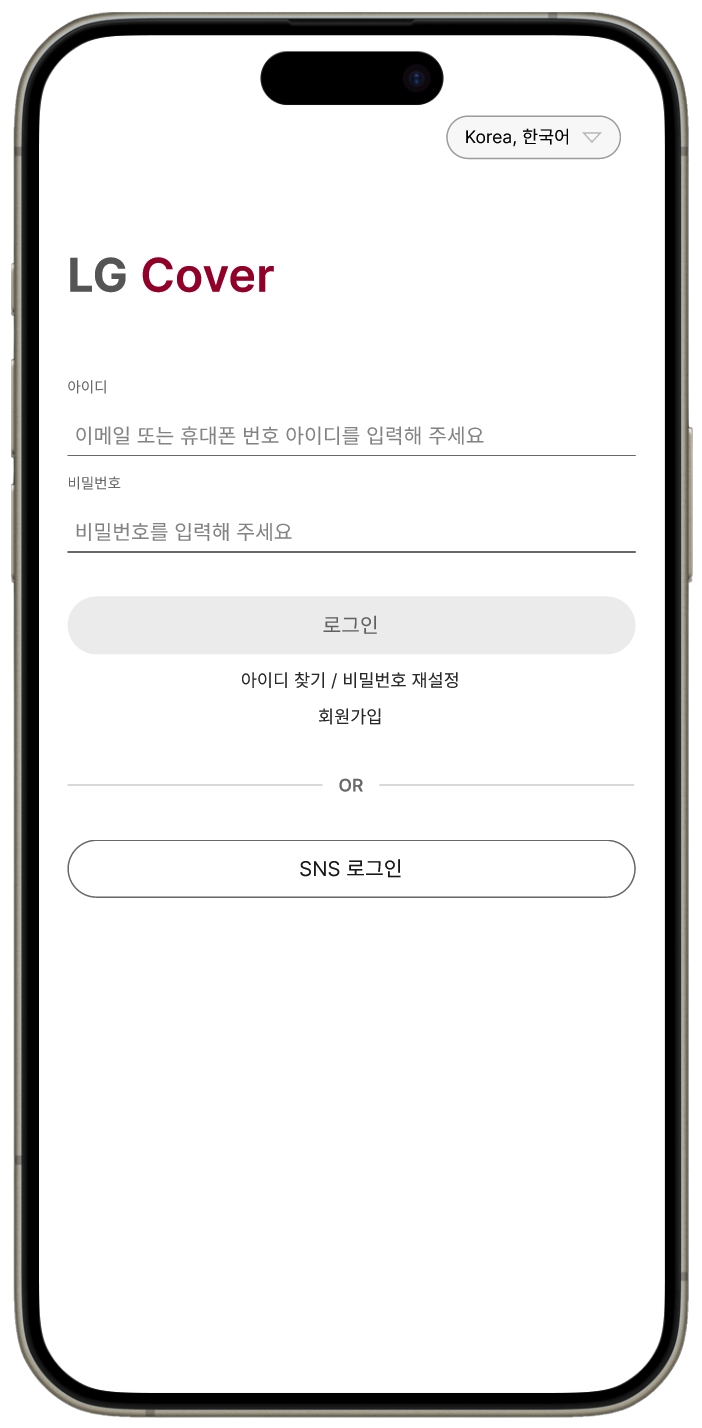
\includegraphics[scale=0.35]{images/sw-spec-1.png}\end{figure}
Upon launching the application, users are greeted by the Login Page, which is the primary gateway for accessing the personalized management features within the app. The Login Page is essential as it ensures secure access for users to control and interact with their devices through the COVER application.\\
To begin, users are prompted to enter their username and password. For new users or those without login credentials, the page provides a series of features: 'Find ID / Reset Password,' 'Sign up,' and 'SNS login' options. The 'Sign up' process is a critical step in gaining access to the app's functionalities, leading users through a streamlined process to create their account.\\
A top right button on the Login Page allows users to customize their experience by selecting their country and language, ensuring that the app meets their regional preferences and language understanding.\\
When users complete the signup and hit the 'Register' button, the system initiates a Register Post API request to the server. Successful completion of this request redirects the user to the Login Page, where they can now log in with their new credentials.\\
The input fields during the signup process have specific constraints to ensure data integrity and user identification. For instance, the name field requires 2 to 5 characters and accepts input directly via the keyboard. The username field permits 5 to 20 characters, allowing only English letters and numbers, while the password field demands 8 to 20 characters, also limited to English letters and numbers, with a re-entry required for confirmation.\\

\item Main Page\\
Upon logging in, the Main Page serves as the user's command center, presenting a comprehensive view of their registered devices within the application. The layout and functionality of this page are tailored to facilitate interaction with the user's smart home ecosystem.\\
\begin{enumerate}[label=\alph*.]
\item Main Page Overview\\
\begin{figure}[H]\centering 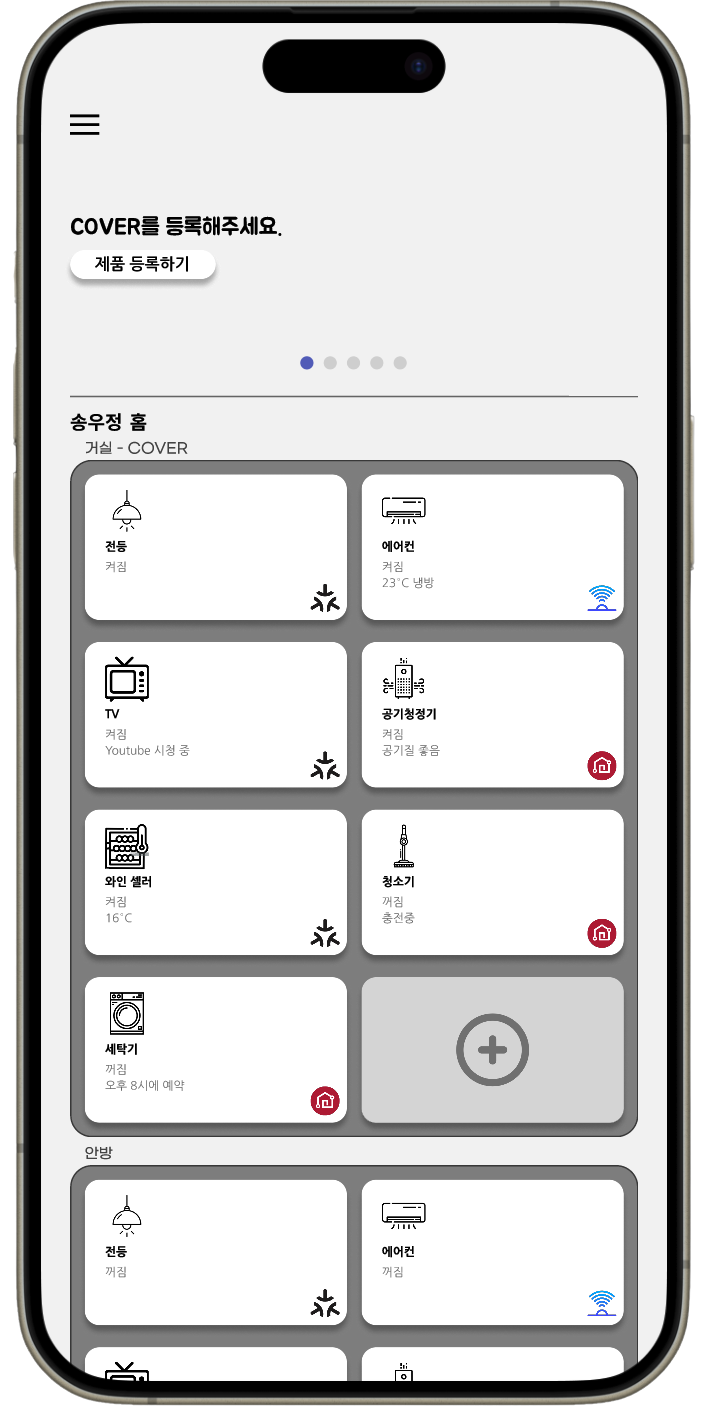
\includegraphics[scale=0.4]{images/sw-spec-2.png}\end{figure}
The Main Page features:\\
\begin{itemize}
\item A display of all the user's registered devices, organized for quick navigation and management.\\
\item Options to manage device settings, monitor device status, add new devices, and link devices to home assistants like Apple Home.\\
\end{itemize}

\item Top Navigation Bar (Top Nav)\\
\begin{figure}[H]\centering 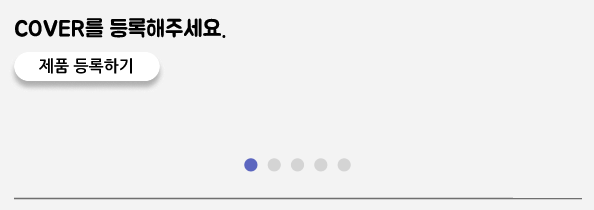
\includegraphics[scale=0.5]{images/sw-spec-3.png}\end{figure}
\begin{figure}[H]\centering 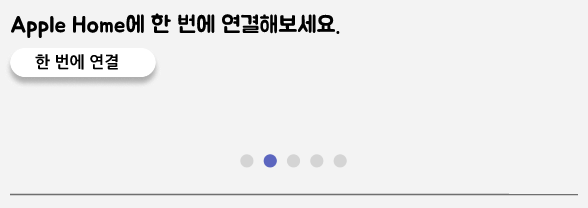
\includegraphics[scale=0.5]{images/sw-spec-4.png}\end{figure}
\begin{itemize}
\item The Top Nav, accessible by swiping horizontally, houses multiple features for device interaction.\\
\item The 'Register Product' menu item leads users to the Device Registration Page, enabling the addition of new devices to the system.\\
\item Additional menu items, revealed by swiping, include shortcuts for quickly connecting all COVER-registered devices to home assistants.\\
\end{itemize}

\item Devide Organization\\
\begin{figure}[H]\centering 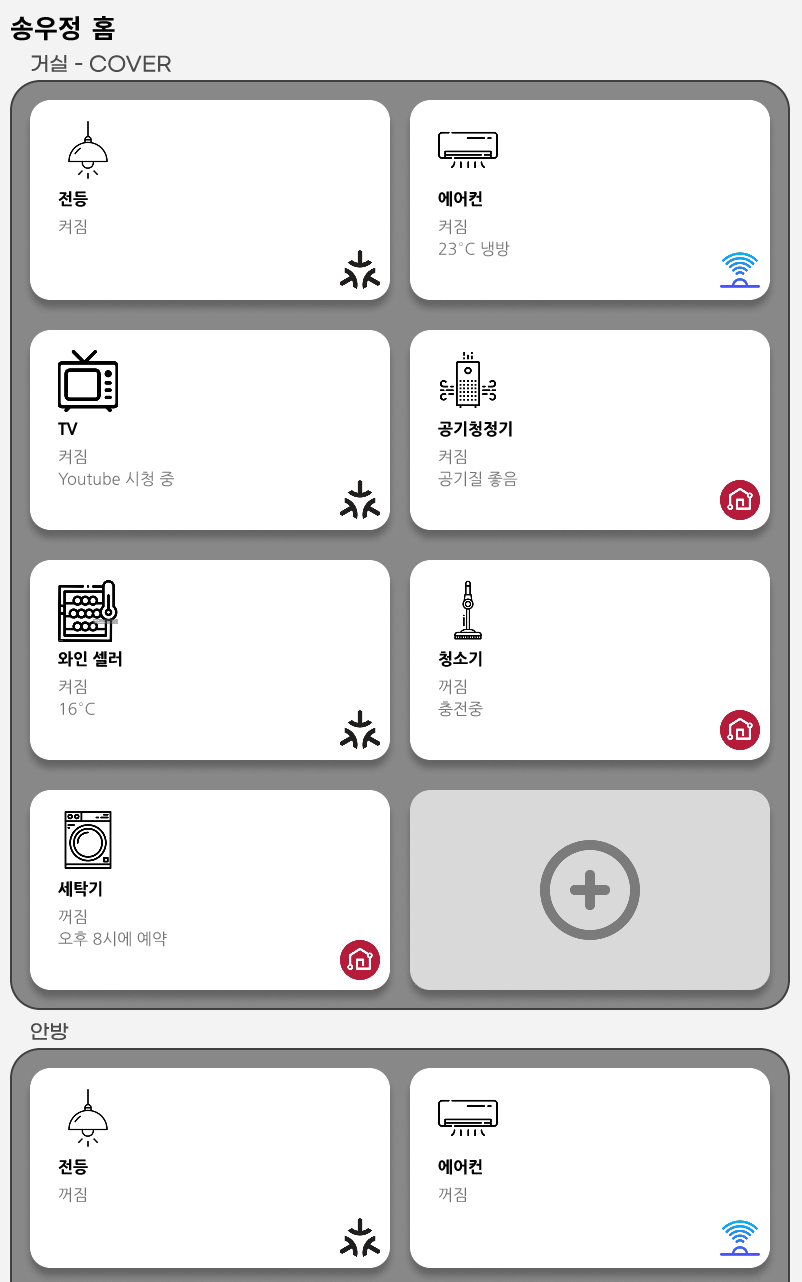
\includegraphics[scale=0.35]{images/sw-spec-5.png}\end{figure}
\begin{itemize}
\item Devices are displayed in a grid layout below the Top Nav, categorized by their physical location (e.g., 'living room') or the hub they are connected to.\\
\item Each device is represented by a tile that includes an icon indicating the device type, the device name, and its current status (e.g., on/off).\\
\item The '+' button at the end of each device category facilitates the registration of new devices to specific locations.\\
\end{itemize}

\item Device Tiles\\
\begin{figure}[H]\centering 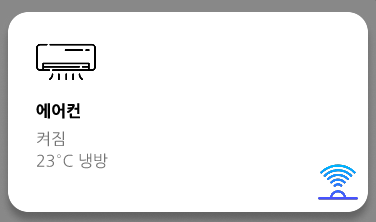
\includegraphics[scale=0.6]{images/sw-spec-6.png}\end{figure}
\begin{figure}[H]\centering 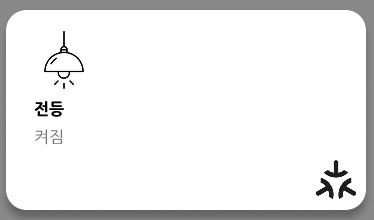
\includegraphics[scale=0.6]{images/sw-spec-7.png}\end{figure}
\begin{figure}[H]\centering 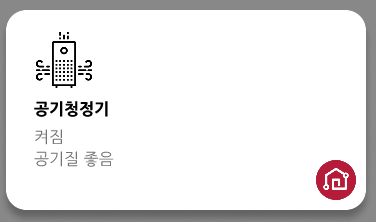
\includegraphics[scale=0.6]{images/sw-spec-8.png}\end{figure}
Device tiles provide at-a-glance information:\\
\begin{itemize}
\item The upper left corner of each tile features a device-specific icon.\\
\item The device name is located just below the icon.\\
\item The current status of the device is displayed, with the available statuses varying by device type.\\
\item The bottom right corner of each tile indicates the device's connection type (Matter, LG ThinQ, or IR), each with a corresponding icon.\\
\begin{table}[ht]
\setlength{\extrarowheight}{2.5pt}
\centering
\begin{tabular}{|c|l|}
\hline
\textbf{Device Type} & \textbf{Status} \\
\hline
Light & On/Off \\
 & Brightness \\
 & Color temperature \\
 & Reservation information \\
\hline
Air Conditioner & On/Off \\
 & Temperature \\
 & Mode \\
 & Reservation information \\
\hline
TV & On/Off \\
 & Currently playing content \\
\hline
Air Purifier & On/Off \\
 & Air quality \\
 & Reservation information \\
\hline
Wine Cellar & On/Off \\
 & Temperature \\
\hline
Vacuum Cleaner & On/Off \\
 & Charging \\
\hline
Washing Machine & On/Off \\
 & Reservation information \\
\hline
\end{tabular}
\end{table}

\end{itemize}

\item Interaction and Design\\
\begin{itemize}
\item The Main Page is designed to be intuitive and user-friendly, allowing for efficient management of the user's smart home devices.\\
\item The interface is clean and organized, ensuring that users can easily find and operate their devices.\\
\item The design is consistent with the application's overall aesthetic, providing a seamless user experience.\\
\end{itemize}
\end{enumerate}


\item Bind with Matter Page\\
\begin{figure}[H]\centering 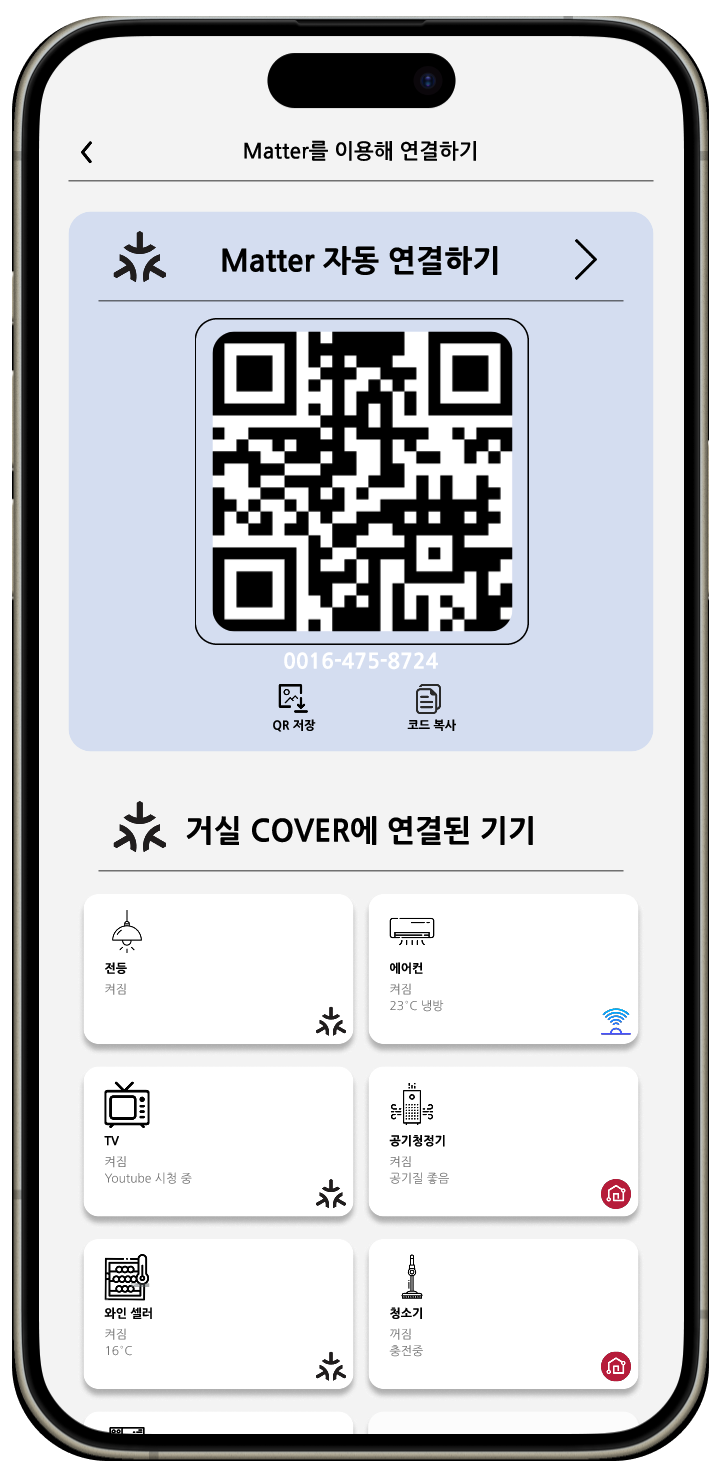
\includegraphics[scale=0.4]{images/sw-spec-9.png}\end{figure}
Upon accessing the Bind with Matter Page within the application, users are presented with a streamlined process to integrate their COVER-managed devices with Apple Home, harnessing the power of the Matter protocol. This page is designed to be a straightforward junction point between COVER and Apple Home, with a couple of pivotal actions available for the user to initiate the integration.\\
Users can secure their setup by using the ‘QR 저장’ button to save the QR code, a crucial step that anchors the device to their account. Alternatively, they can use the ‘코드 복사’ button to copy the COVER setup code, allowing for a manual connection if needed. These options cater to different user preferences, ensuring versatility in the setup process.\\
Advancing in the setup, the ‘Matter 자동 연결하기’ button is a significant feature on this page. With a simple press, users command the application to proceed with the automatic registration of COVER to Apple Home. This button effectively initiates a seamless transition to Apple Home’s accessory addition page, where the previously registered devices on COVER become part of the Apple Home ecosystem, ready for centralized control.\\
However, users must be aware of certain limitations inherent to the system's design. Notably, when connecting COVER with Apple Home through Matter, there is a cap on the number of devices that can be managed. The system currently supports a maximum of 30 devices linked to COVER. This limit is set to ensure that each device maintains a robust and reliable connection within the smart home network. Attempting to add more than 30 devices could lead to potential performance issues, affecting both the new and existing devices' functionality.\\
This limitation emphasizes the importance of strategic planning in the user's smart home setup. For those users who wish to exceed the 30-device threshold, exploring additional configurations, such as incorporating another hub, may be necessary to distribute the network load and maintain system integrity.\\
In conclusion, the Bind with Matter Page serves as a gateway for users to expand and centralize their smart home control within Apple Home. While designed for ease of use and convenience, it operates within the defined device limitation to ensure optimal performance across the smart home network. Users should navigate this page with an understanding of these parameters to fully leverage the capabilities of their COVER and Apple Home integrated experience.\\
\begin{figure}[H]\centering 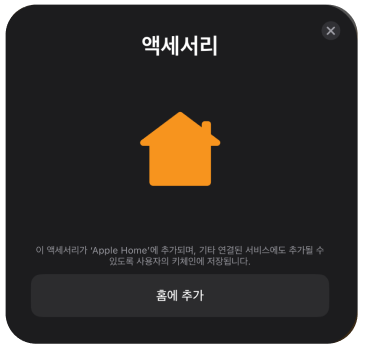
\includegraphics[scale=0.5]{images/sw-spec-10.png}\end{figure}

\item Device Registration Page\\
The Device Registration Page acts as the gateway for incorporating new devices into the user's smart home setup, featuring a methodical and comprehensive approach for adding devices via various protocols like Matter, LG ThinQ, and Infrared (IR).\\
\begin{enumerate}[label=\alph*.]
\item Matter and LG ThinQ Device Registration\\
\begin{figure}[H]\centering 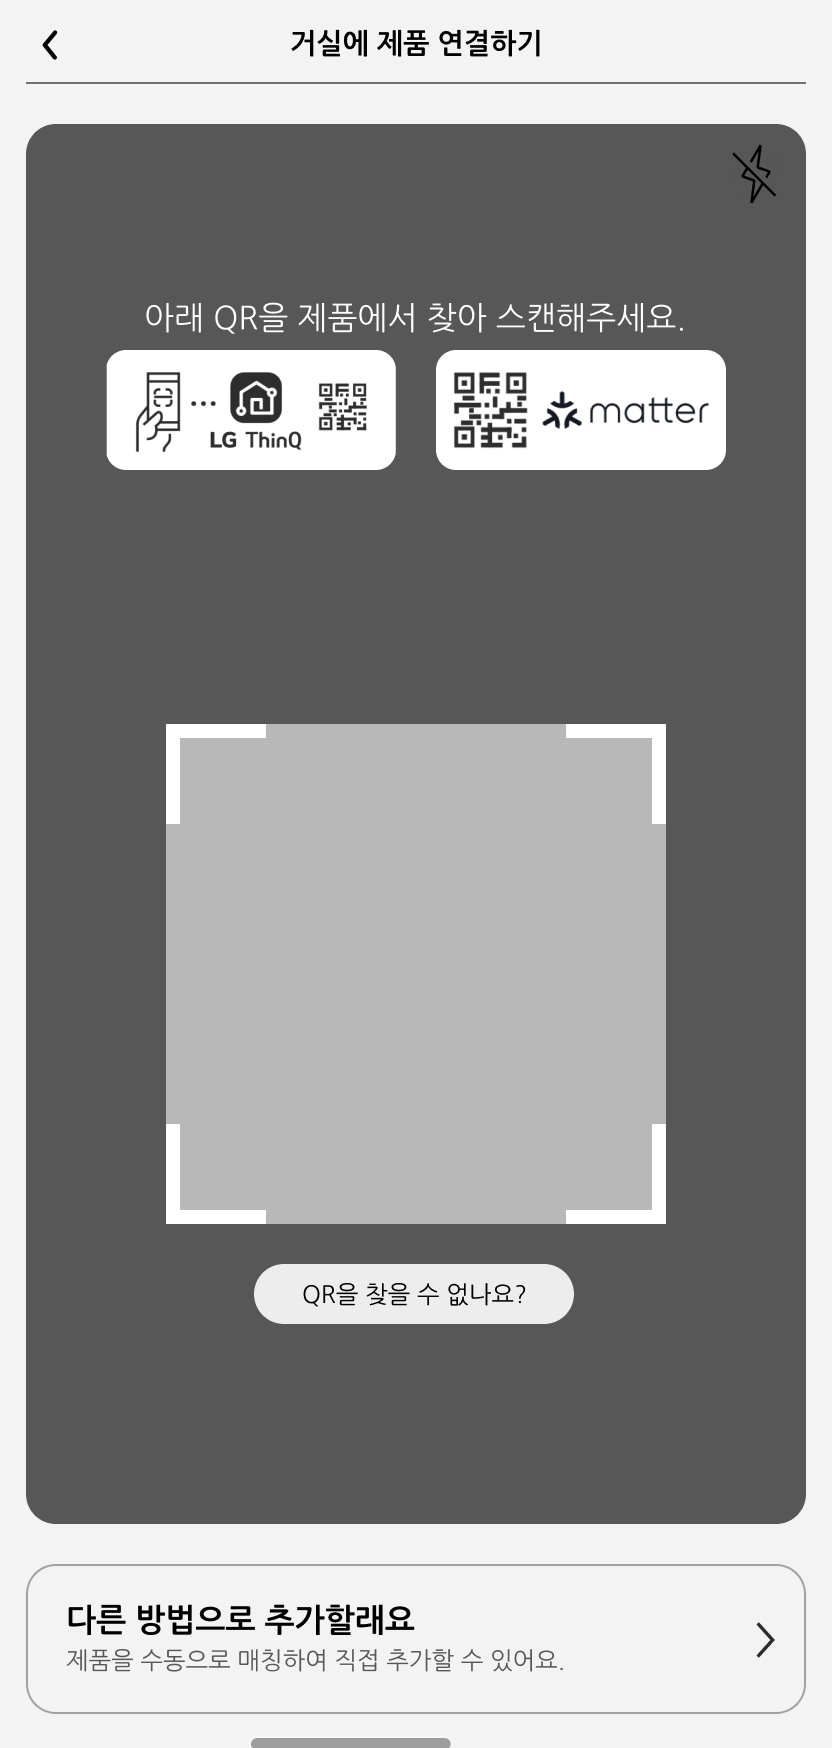
\includegraphics[scale=0.35]{images/sw-spec-11.png}\end{figure}
Upon landing on the Device Registration Page, users are prompted to register their Matter or LG ThinQ devices by scanning a QR code. The page activates the camera on the user's mobile device, allowing for the QR code to be read seamlessly. The system is intuitive enough to distinguish between a Matter QR code and an LG ThinQ QR code:\\
\begin{itemize}
\item \textbf{For Matter Devices}: The system, upon recognizing a Matter device's QR code, proceeds to automatically add the device to the user’s profile, integrating it into the smart home network without additional steps.\\
\item \textbf{For LG ThinQ Devices}: If the QR code corresponds to an LG ThinQ device, the user is redirected to a specialized LG ThinQ Registration Page. This page not only displays the device's specifics, such as its type and model name, but also an image for visual confirmation. Here, the user can finalize the registration by pressing the '추가하기' button. This action triggers the system to store all relevant information, including control commands and status features, within LG's comprehensive database. Subsequently, COVER gains access to these details, allowing the user to manage the device via the COVER interface.\\
\begin{figure}[H]\centering 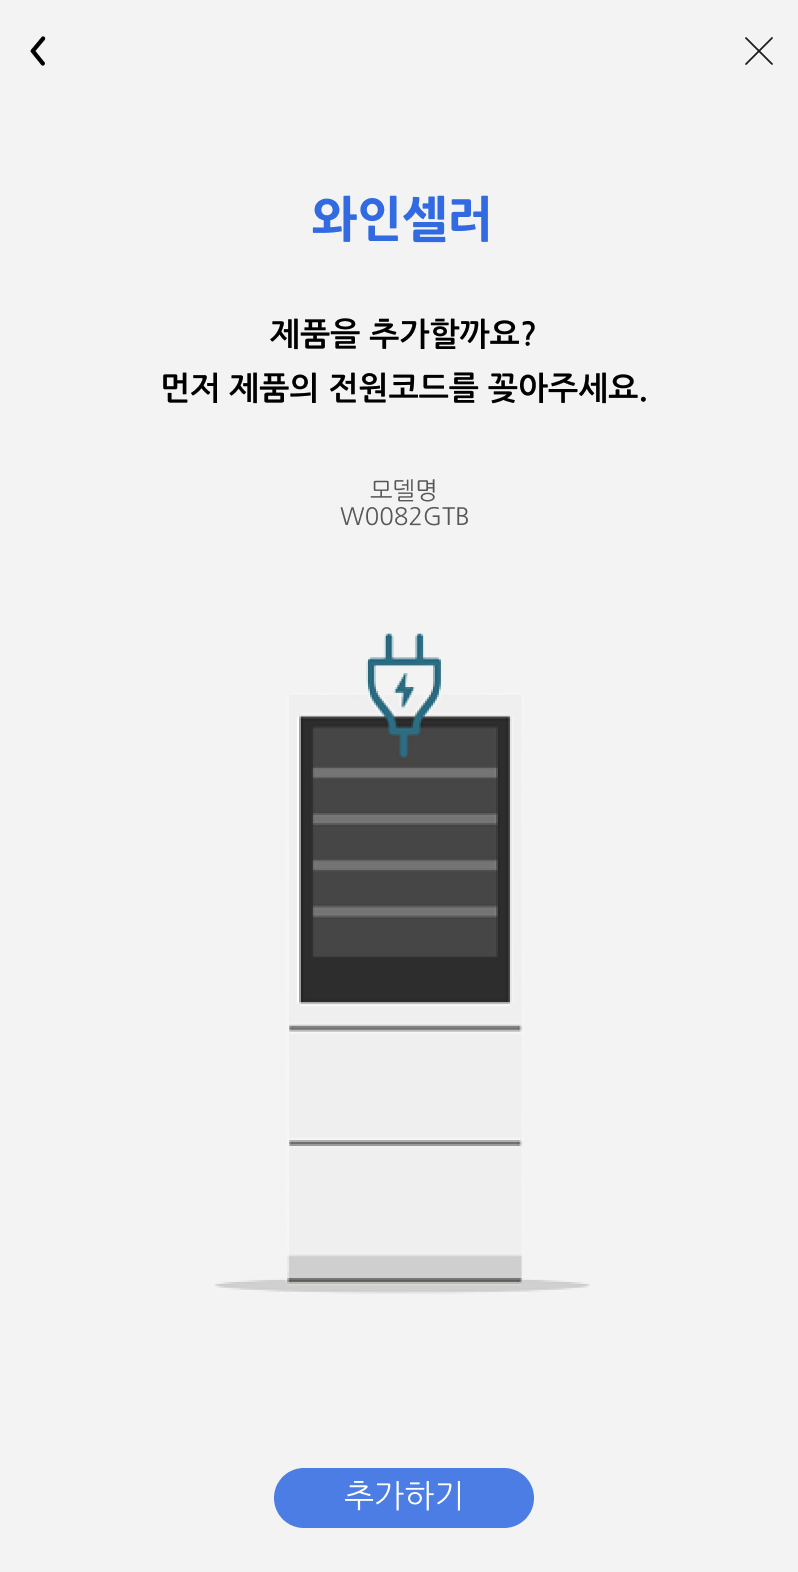
\includegraphics[scale=0.35]{images/sw-spec-12.png}\end{figure}
\end{itemize}
\item IR Device Registration\\
\begin{figure}[H]\centering 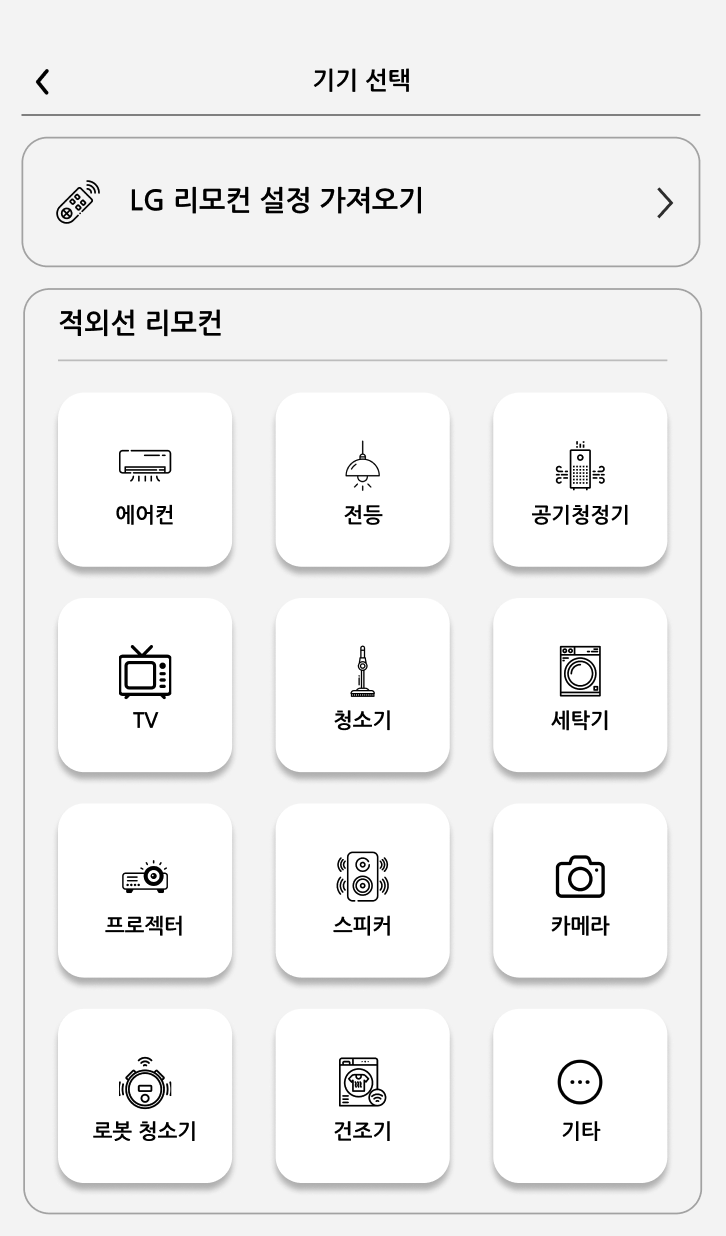
\includegraphics[scale=0.35]{images/sw-spec-13.png}\end{figure}
For devices that operate via IR, especially those that do not support QR code scanning, the registration process is facilitated through an alternative method:\\
\begin{itemize}
\item \textbf{For LG IR Devices}: Users can initiate the setup by clicking the ‘다른 방법으로 추가할래요’ (Add in another way) button, which redirects them to the IR Registration Page. If the IR device is manufactured by LG, users can fetch the remote control settings from LG's database by pressing the ‘LG 리모컨 설정 가져오기’ (Retrieve LG remote control settings) button. The system then presents a list of devices matching the entered serial number from which the user can select the appropriate one.\\
\begin{figure}[H]\centering 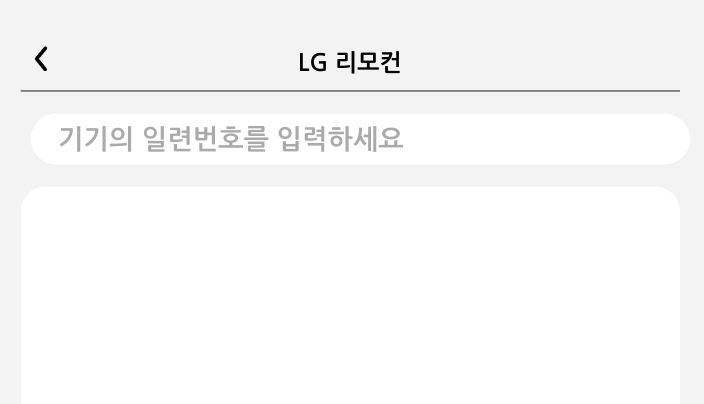
\includegraphics[scale=0.5]{images/sw-spec-14.png}\end{figure}
\item \textbf{For Non-LG IR Devices}: When dealing with non-LG IR devices, the process requires the user to manually transmit the IR signal from the device's remote control to COVER. This is done by selecting the type of device they wish to register and following the prompts to transmit each function's corresponding signal. For instance, if registering a lighting device, COVER's interface will guide the user to input signals for power, brightness, and color temperature adjustments. As the user matches and transmits these signals, they are captured and stored by COVER for future command executions.\\
\begin{figure}[H]\centering 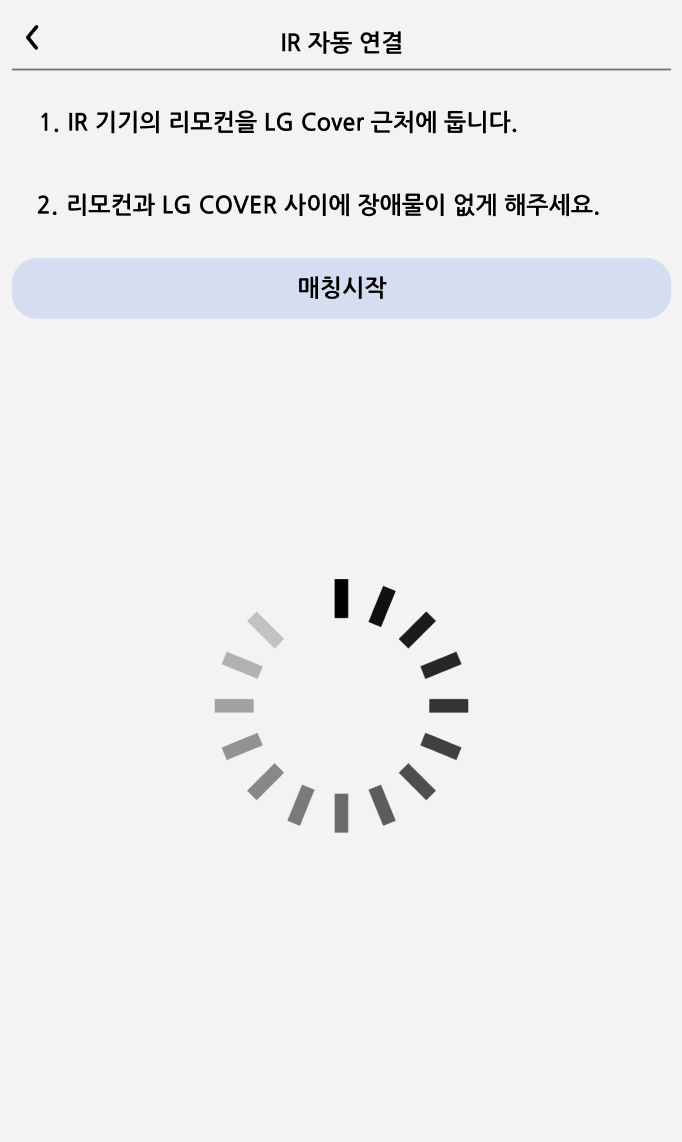
\includegraphics[scale=0.4]{images/sw-spec-15.png}\end{figure}
During the IR signal transmission process, the user is provided with a visual indicator, such as a loading bar, to denote the progress of the signal capture. Once a signal is successfully stored, the interface is designed to revert to the remote control display, enabling the user to proceed with storing additional signals for different commands.\\
\begin{figure}[H]\centering 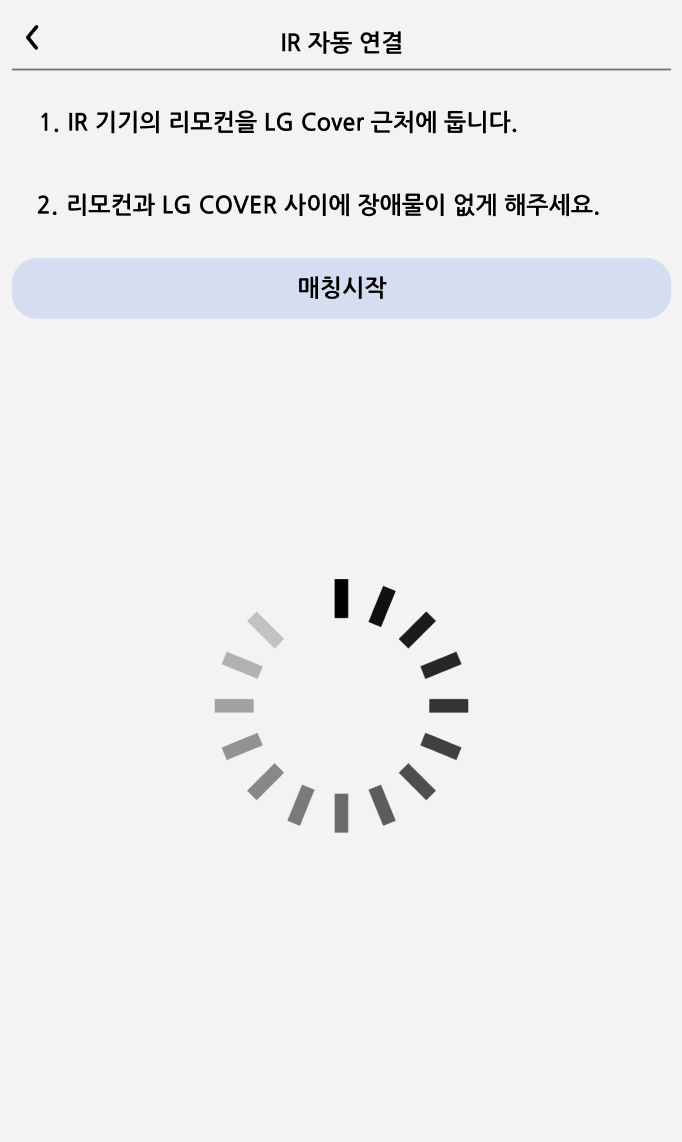
\includegraphics[scale=0.4]{images/sw-spec-16.png}\end{figure}
\end{itemize}
\end{enumerate}
\end{enumerate}



\subsection{\large{User Documentation}}
\begin{enumerate}[label=\arabic*.]
\item Compliance with Matter standards.\\
\item Secure QR code generation and scanning.\\
\item Robust error handling for failed device additions or communications.\\
\item Thorough testing with various brands and types of devices to ensure compatibility.\\
\end{enumerate}

\subsection{\large{Quality Assurance}}
\begin{enumerate}[label=\arabic*.]
\item Detailed setup guide for LG Cover and device registration.\\
\item Troubleshooting tips for common issues during setup or use.\\
\item Contact information for support.\\
\end{enumerate}


\begin{thebibliography}{00}
\bibitem{b1} Smart Home Market Revenue Trends and growth drivers - 2023. MarketsandMarkets. https://www.marketsandmarkets.com/Market-Reports/smart-homes-and-assisted-living-advanced-technologie-and-global-market-121.html?gclid=EAIaIQobChMImsWklrrwgQMV62sPAh2Blg4VEAAY\\ASAAEgLVQfD\_BwE \\
\bibitem{b2} 2019 Digital America State of the U.S. Consumer Electronics Industry. https://cdn.cta.tech/cta/media/media/resources/i3/pdfs/digital-america-2019.pdf \\
\bibitem{b3} Ding, J., Nemati, M., Ranaweera, C., \& Choi, J. (2020). IoT Connectivity Technologies and Applications: A Survey. IEEE Access, 8, 67646-67673.\\
\bibitem{b4} Shah, S.K., \& Mahmood, W. (2020). Smart Home Automation Using IOT and its Low Cost Implementation. International Journal of Engineering and Manufacturing, 10, 28-36.\\
\bibitem{b5} Iqbal, W., Abbas, H., Daneshmand, M., Rauf, B., \& Bangash, Y.A. (2020). An In-Depth Analysis of IoT Security Requirements, Challenges, and Their Countermeasures via Software-Defined Security. IEEE Internet of Things Journal, 7, 10250-10276.
\bibitem{b6} Espressif Systems. (2023). esp-idf: Espressif IoT Development Framework [Software]. GitHub. Retrieved November 10, 2023, from https://github.com/espressif/esp-idf\\
\bibitem{b7} Espressif Systems. (n.d.). About - ESP-IDF Programming Guide. Retrieved November 9, 2023, from https://docs.espressif.com/projects/esp-idf/en/latest/esp32s3/about.html\\
\bibitem{b8} Kitware. (2023). The standard build system - CMake. Retrieved November 9, 2023, from https://cmake.org/features/\\
\bibitem{b9} Ninja. (n.d.). [Home page]. Ninja-build.org. Retrieved November 9, 2023, from https://ninja-build.org/\\
\bibitem{b10} React Native. (2023). [Home page]. Reactnative.dev. Retrieved November 9, 2023, from https://reactnative.dev/\\
\bibitem{b11} Go. (n.d.). [Home page]. Go.dev. Retrieved November 9, 2023, from https://go.dev\\
\bibitem{b12} LG. (2023). LG ThinQ. Retrieved November 9, 2023, from https://www.lg.com/us/lg-thinq\\
\bibitem{b13} Microsoft. (2023). [Home page]. Visual Studio Code. Retrieved November 9, 2023, from https://code.visualstudio.com/\\
\end{thebibliography}

\end{document}
